\documentclass[10pt, aspectratio=169]{beamer}

% Paquetes básicos
\usepackage[utf8]{inputenc}
\usepackage[spanish]{babel}
\usepackage{amsmath, amssymb}
\usepackage{graphicx}
\usepackage{booktabs}
\usepackage{caption}

% Tema visual
\usetheme{Madrid}
\usecolortheme{default}
\graphicspath{{img/}}

% Información del título
\title[Salud en la esfera pública]{Salud en la esfera pública}
\subtitle{Resultados del análisis del subcorpus de salud en tweets en español}
\author{Andrés F. Puerta}
\date{2026}

\begin{document}

% ---------------------------------------------------
% Diapositiva 1: Título
\begin{frame}
    \titlepage
\end{frame}

% ---------------------------------------------------
% Diapositiva 2: Contexto y metodología
\begin{frame}{Contexto y metodología}

  \begin{columns}[T]
    \column{0.5\textwidth}
      \textbf{Objetivo}
      \begin{itemize}
        \item Caracterizar c\'omo se habla de \textbf{salud}
              en un corpus de tweets en espa\~nol.
        \item Identificar qu\'e actores, instituciones,
              enfermedades y medicamentos aparecen con
              mayor frecuencia.
        \item Describir la evoluci\'on temporal y tem\'atica
              del subcorpus de salud.
      \end{itemize}

    \column{0.5\textwidth}
      \textbf{Pipeline aplicado}
      \begin{enumerate}
        \item Preprocesamiento y selecci\'on del subcorpus
              de salud (umbral de similitud sem\'antica).
        \item Descriptivos generales: autores, tipo de
              cuenta, evoluci\'on mensual.
        \item Subcategor\'ias tem\'aticas de salud
              (13 categor\'ias).
        \item NER (entidades), POS (verbos, sustantivos,
              adjetivos), BERTopic.
        \item B\'usqueda dirigida: lugares, instituciones,
              enfermedades, medicamentos, figuras clave.
      \end{enumerate}
  \end{columns}

\end{frame}

% ---------------------------------------------------
% Diapositiva 3: Distribución de tweets de salud por autor
\begin{frame}{Descriptivos generales: distribuci\'on por autor}

  \begin{columns}[T]
    \column{0.55\textwidth}
      \begin{figure}
        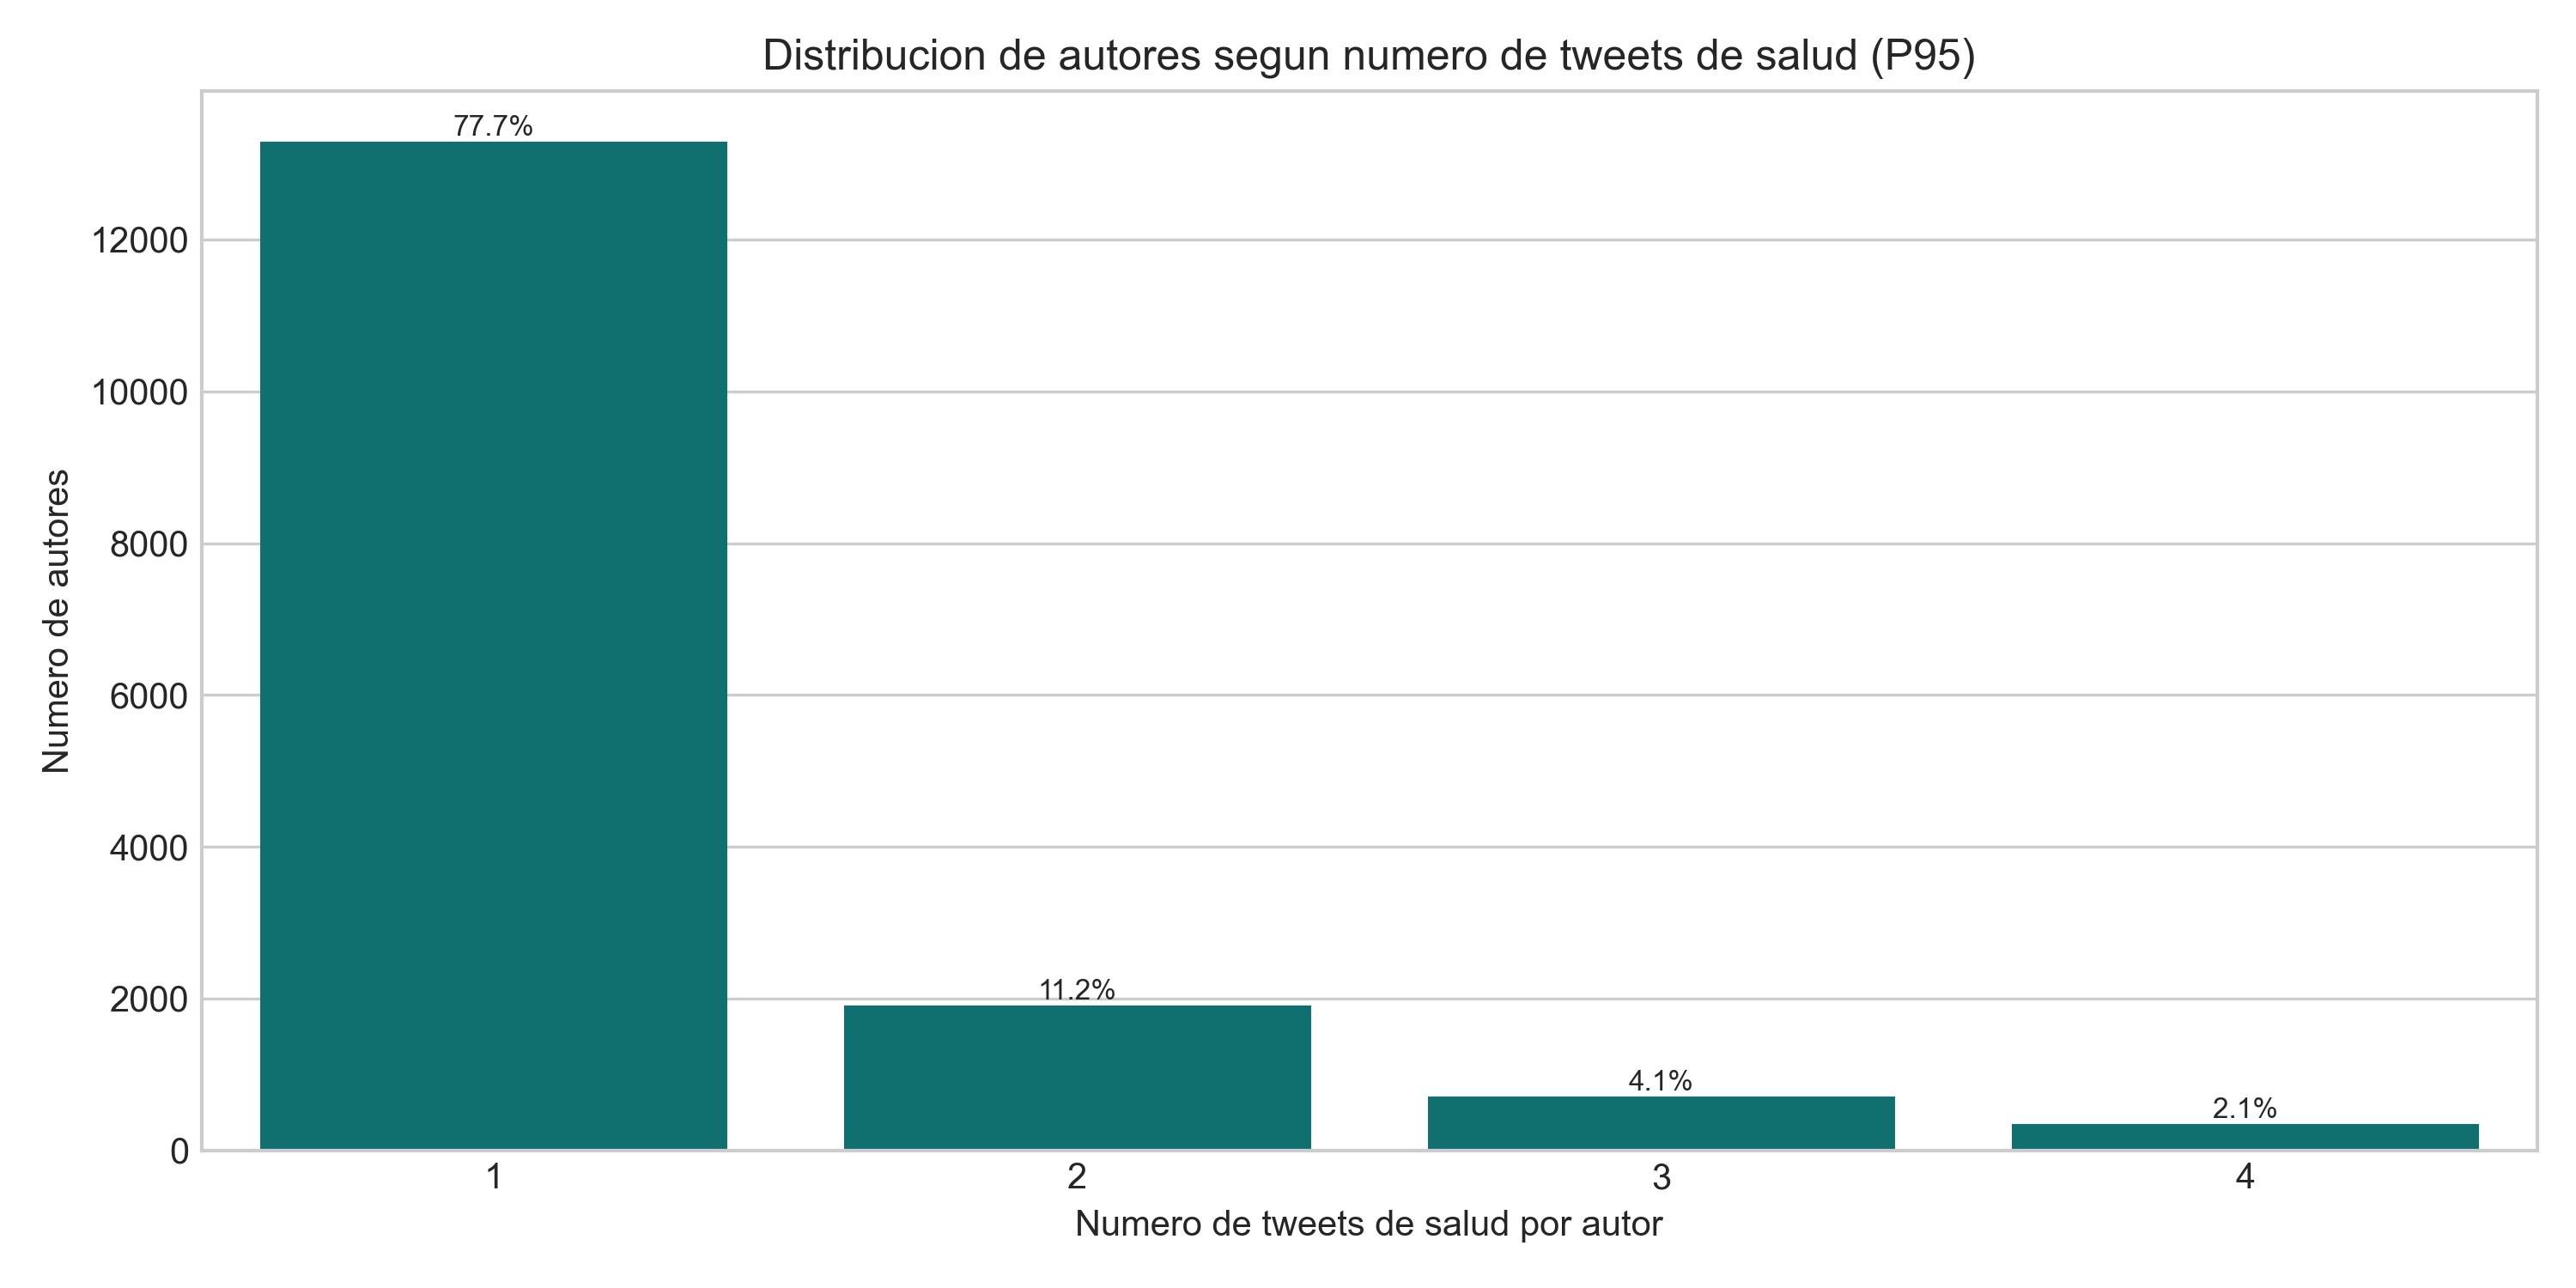
\includegraphics[width=\linewidth]{fig_dist_tweets_salud_por_autor.png}
      \end{figure}

    \column{0.42\textwidth}
      \textbf{Lectura del gr\'afico}\\[6pt]
      Distribuci\'on de autores seg\'un cu\'antos tweets
      sobre salud publicaron (hasta el percentil 95).

      \bigskip
      \begin{itemize}
        \item La mayor\'ia de autores publica
              \alert{muy pocos} tweets sobre salud.
        \item Una minor\'ia de autores concentra un
              n\'umero mucho mayor de menciones.
        \item Patr\'on t\'ipico de distribuci\'on
              de cola larga en redes sociales.
      \end{itemize}
  \end{columns}

\end{frame}

% ---------------------------------------------------
% Diapositiva 4: Evolución temporal (barras y línea)
\begin{frame}{Evoluci\'on temporal de las menciones de salud}

  \begin{columns}[T]
    \column{0.5\textwidth}
      \begin{figure}
        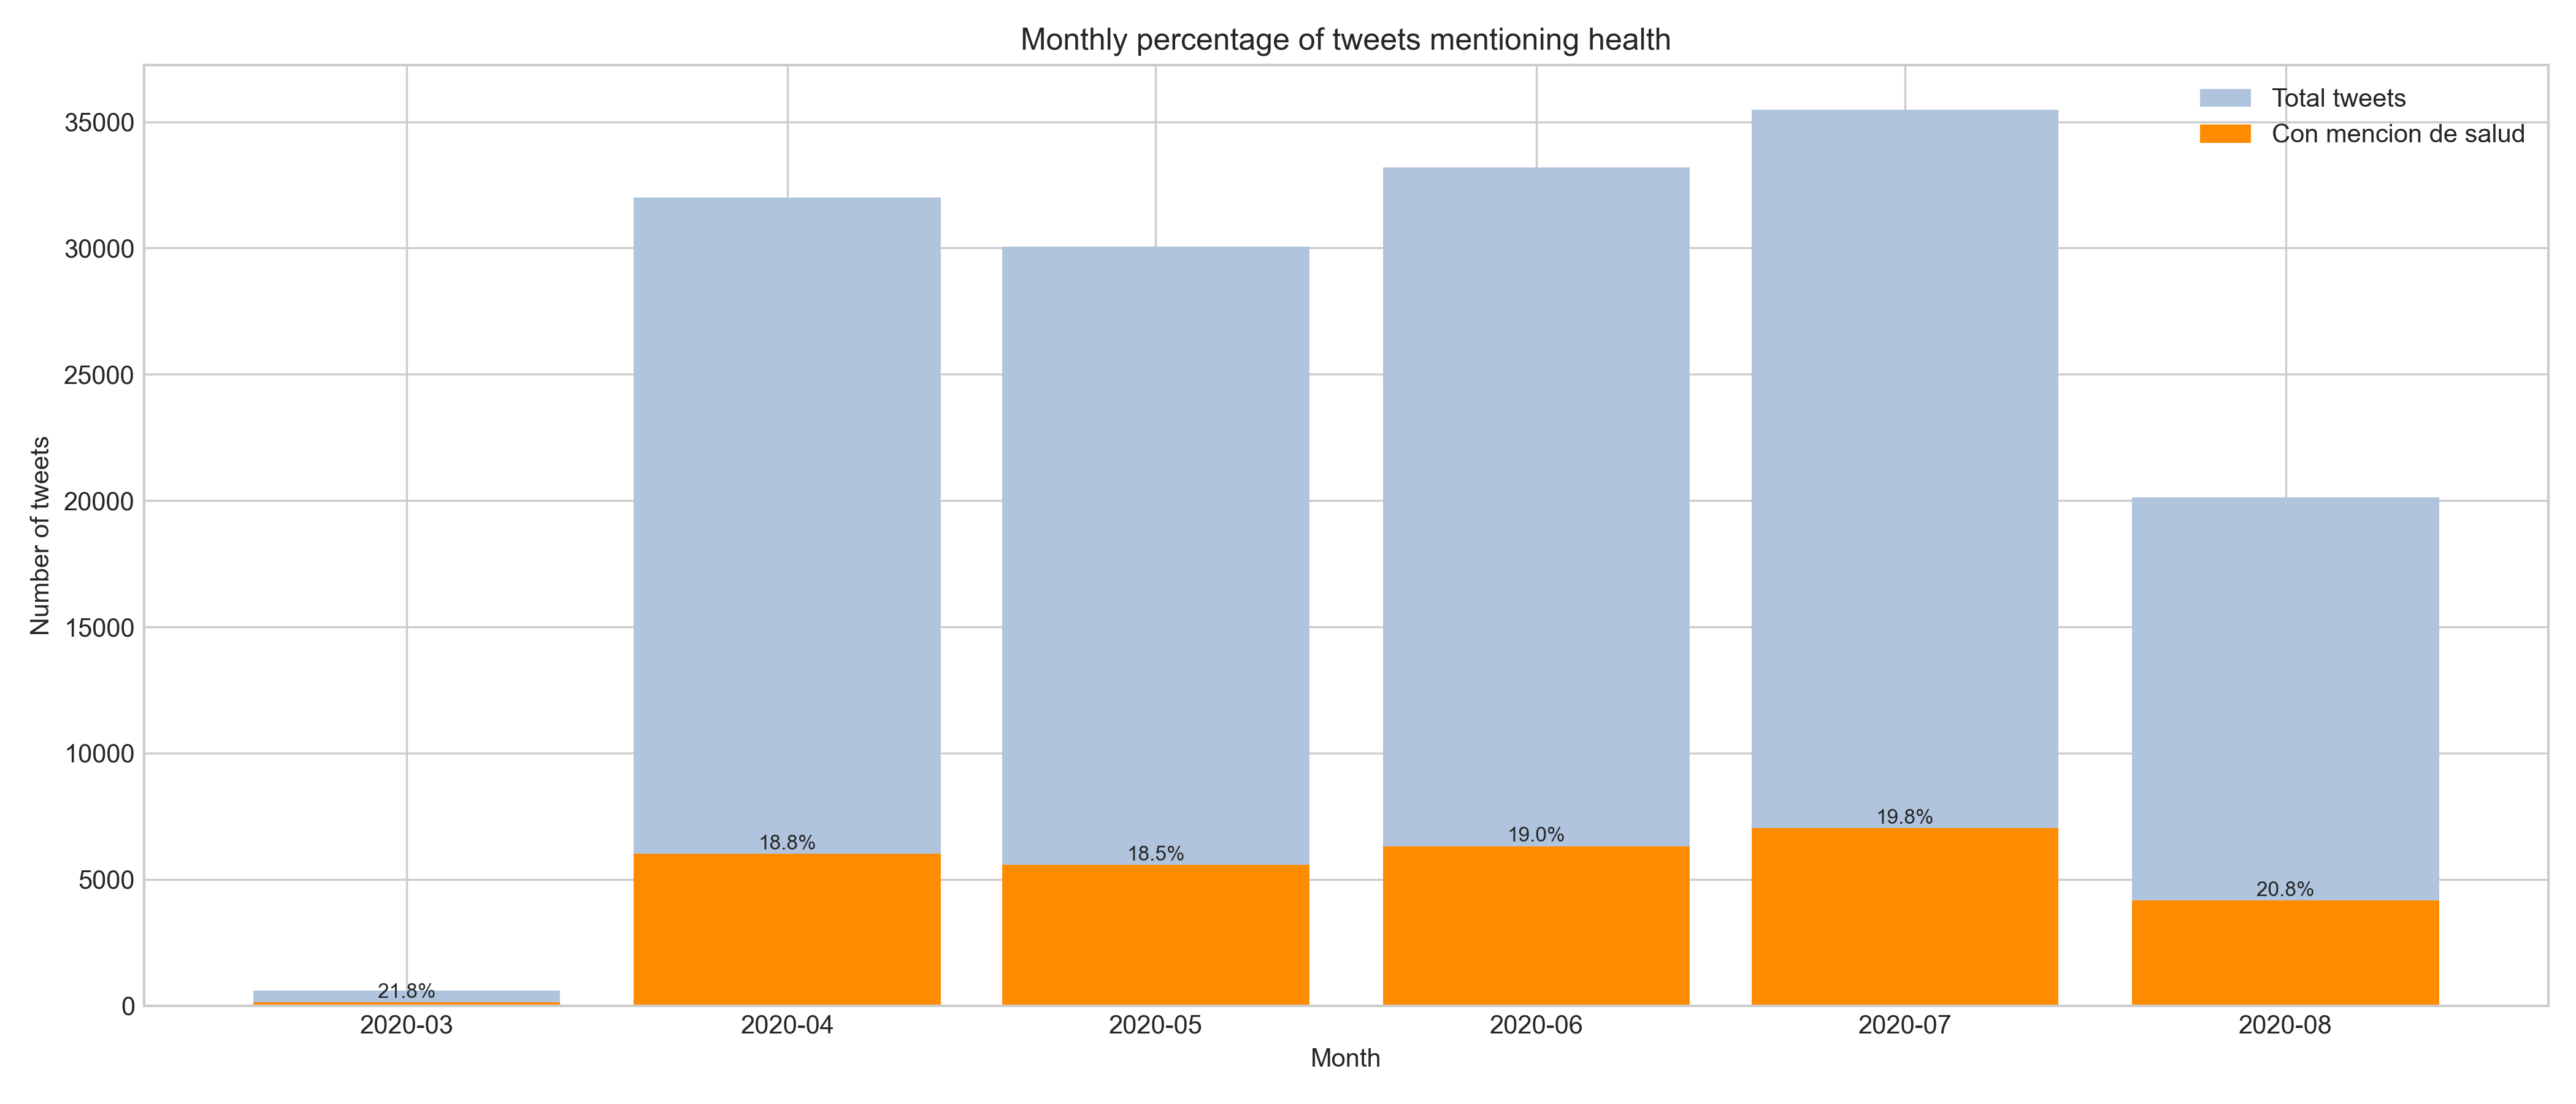
\includegraphics[width=\linewidth]{fig_porcentaje_mensual_salud_barras.png}
        \caption*{\small Tweets totales vs.\ tweets con menci\'on de salud, por mes}
      \end{figure}

    \column{0.5\textwidth}
      \begin{figure}
        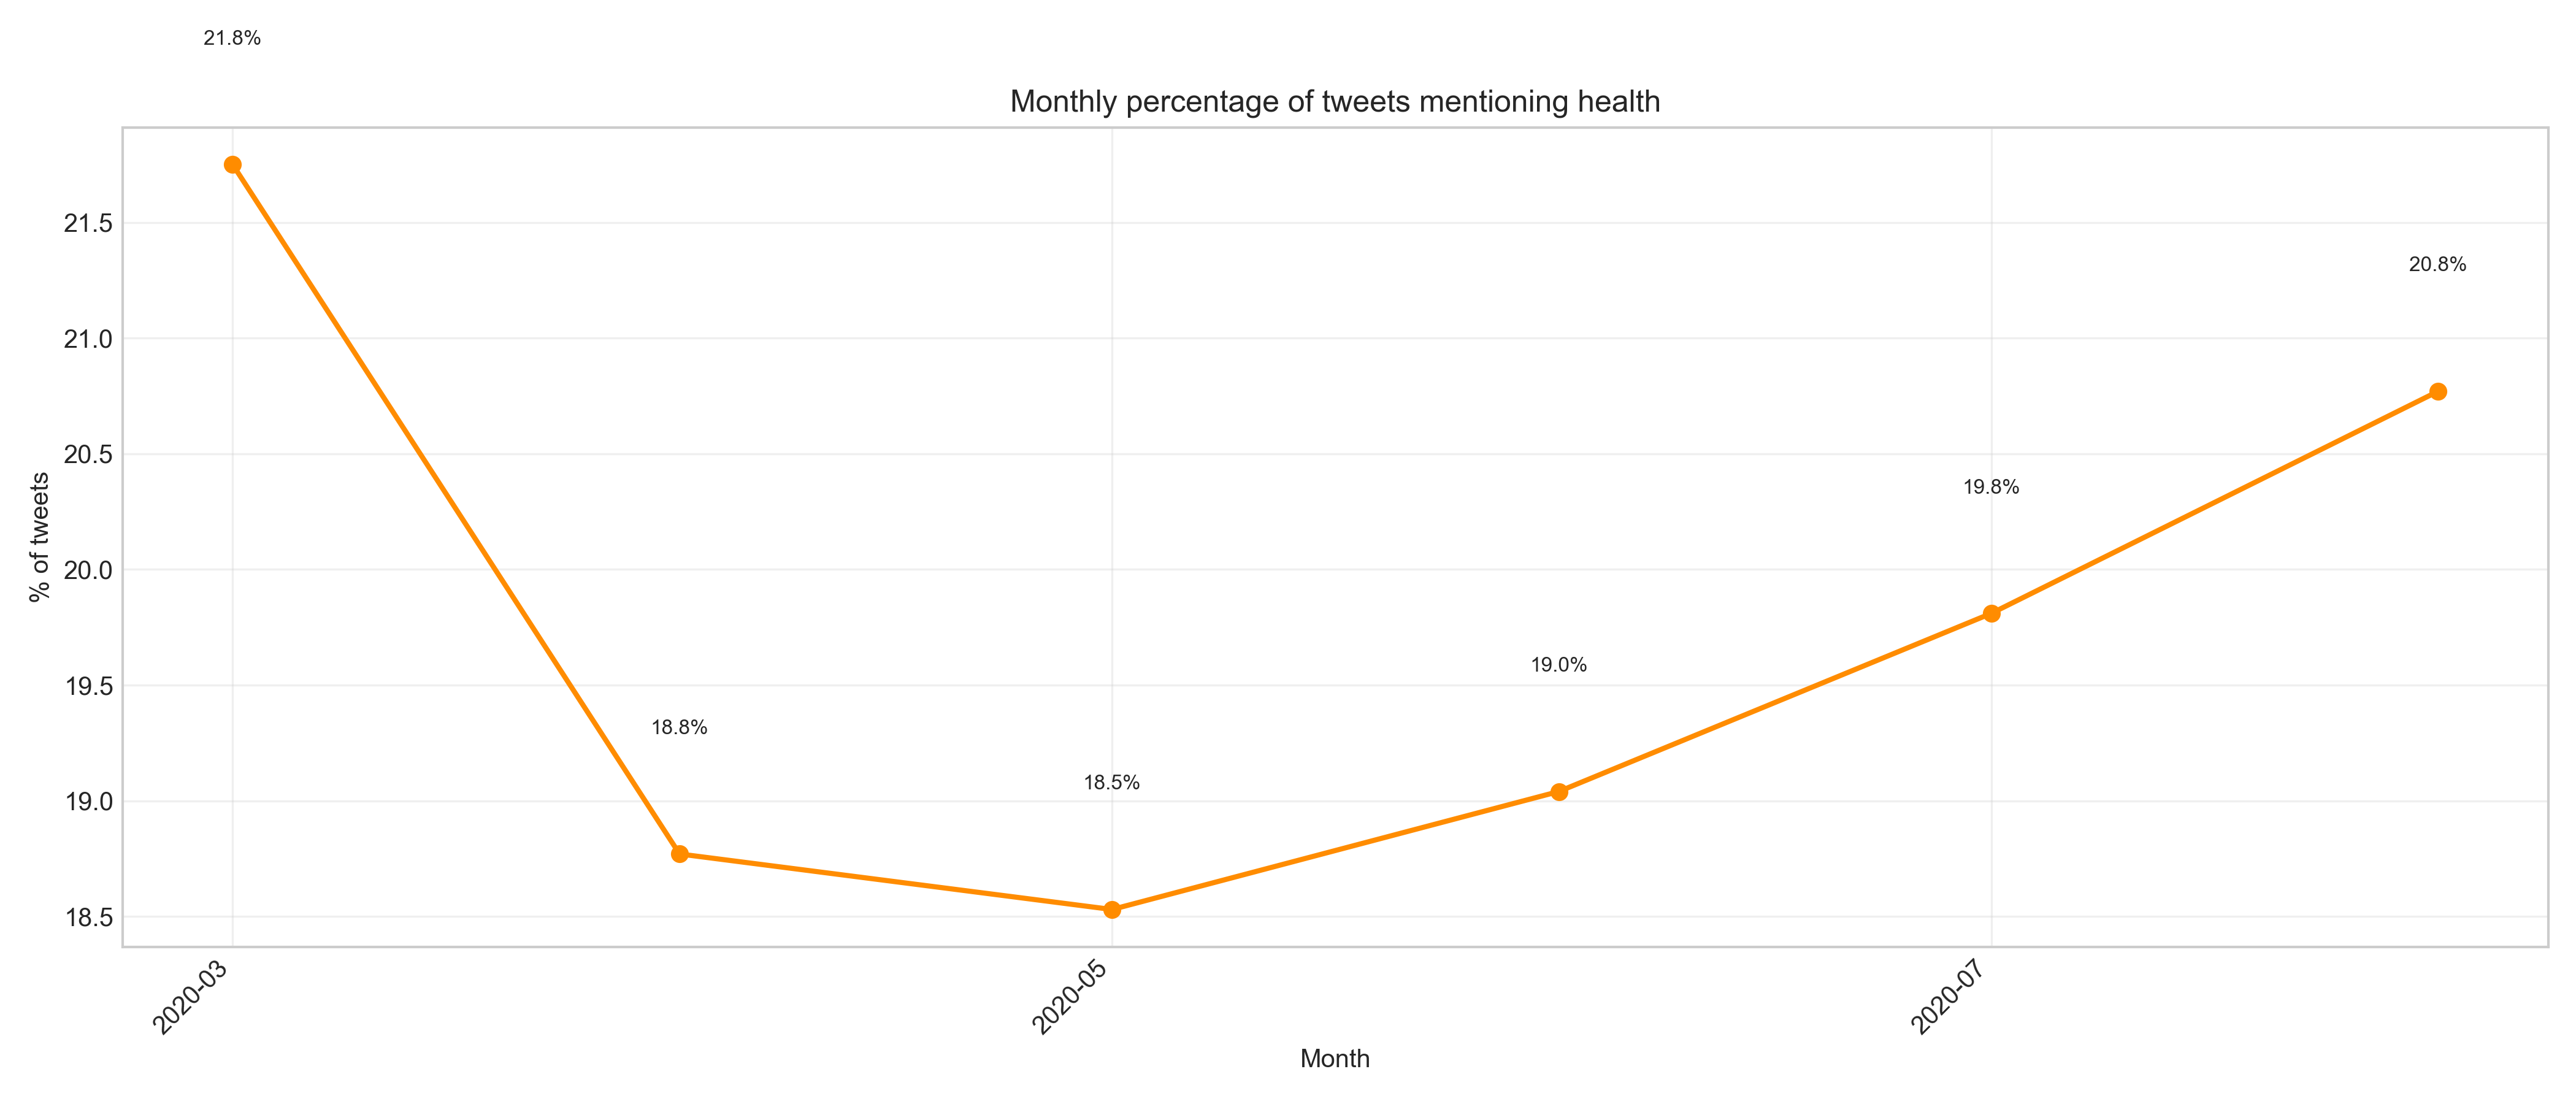
\includegraphics[width=\linewidth]{fig_porcentaje_mensual_salud_linea.png}
        \caption*{\small Porcentaje mensual de tweets con menci\'on de salud}
      \end{figure}
  \end{columns}

  \medskip
  \begin{itemize}
    \item El volumen de menciones de salud var\'ia
          considerablemente mes a mes.
    \item Se observan picos asociados a periodos de
          mayor atenci\'on medi\'atica al tema de salud.
  \end{itemize}

\end{frame}

% ---------------------------------------------------
% Diapositiva 5: Evolución temporal (versión avanzada)
\begin{frame}{Evoluci\'on temporal: porcentaje mensual (vista agregada)}

  \begin{figure}
    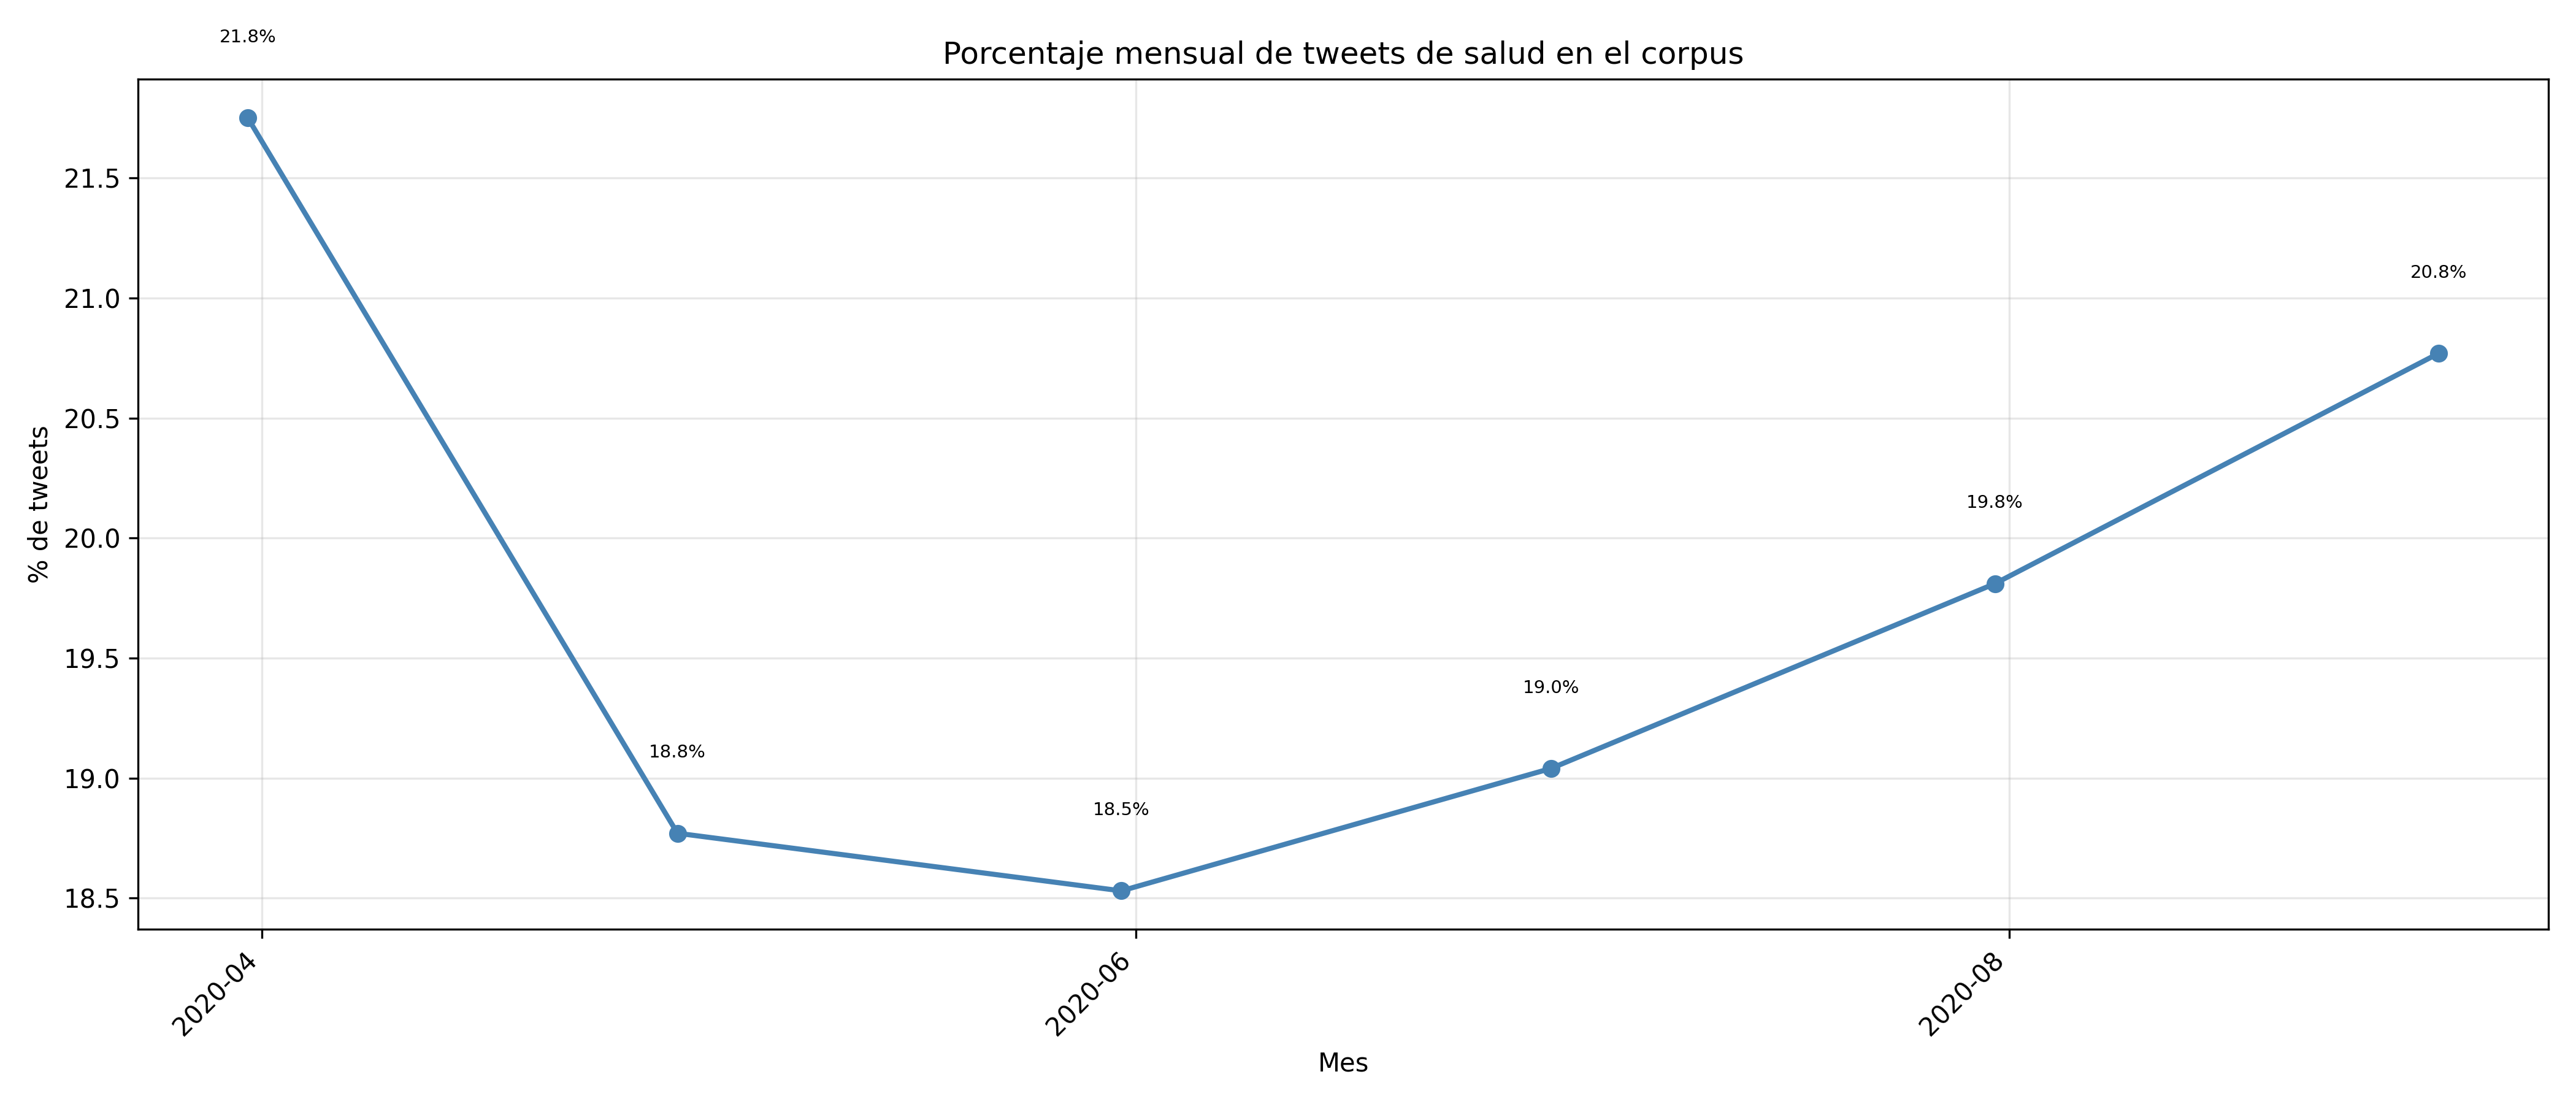
\includegraphics[width=0.85\linewidth]{fig_porcentaje_mensual_salud_avanzado.png}
  \end{figure}

  \begin{center}
  \small
  Replica del an\'alisis anterior con agregaci\'on mensual
  completa, mostrando el porcentaje que representan los
  tweets de salud sobre el total del corpus a lo largo
  de todo el periodo analizado.
  \end{center}

\end{frame}

% ---------------------------------------------------
% Diapositiva 6: Autores con más tweets de salud
\begin{frame}{Autores con m\'as tweets sobre salud}

  \begin{columns}[T]
    \column{0.5\textwidth}
      \begin{figure}
        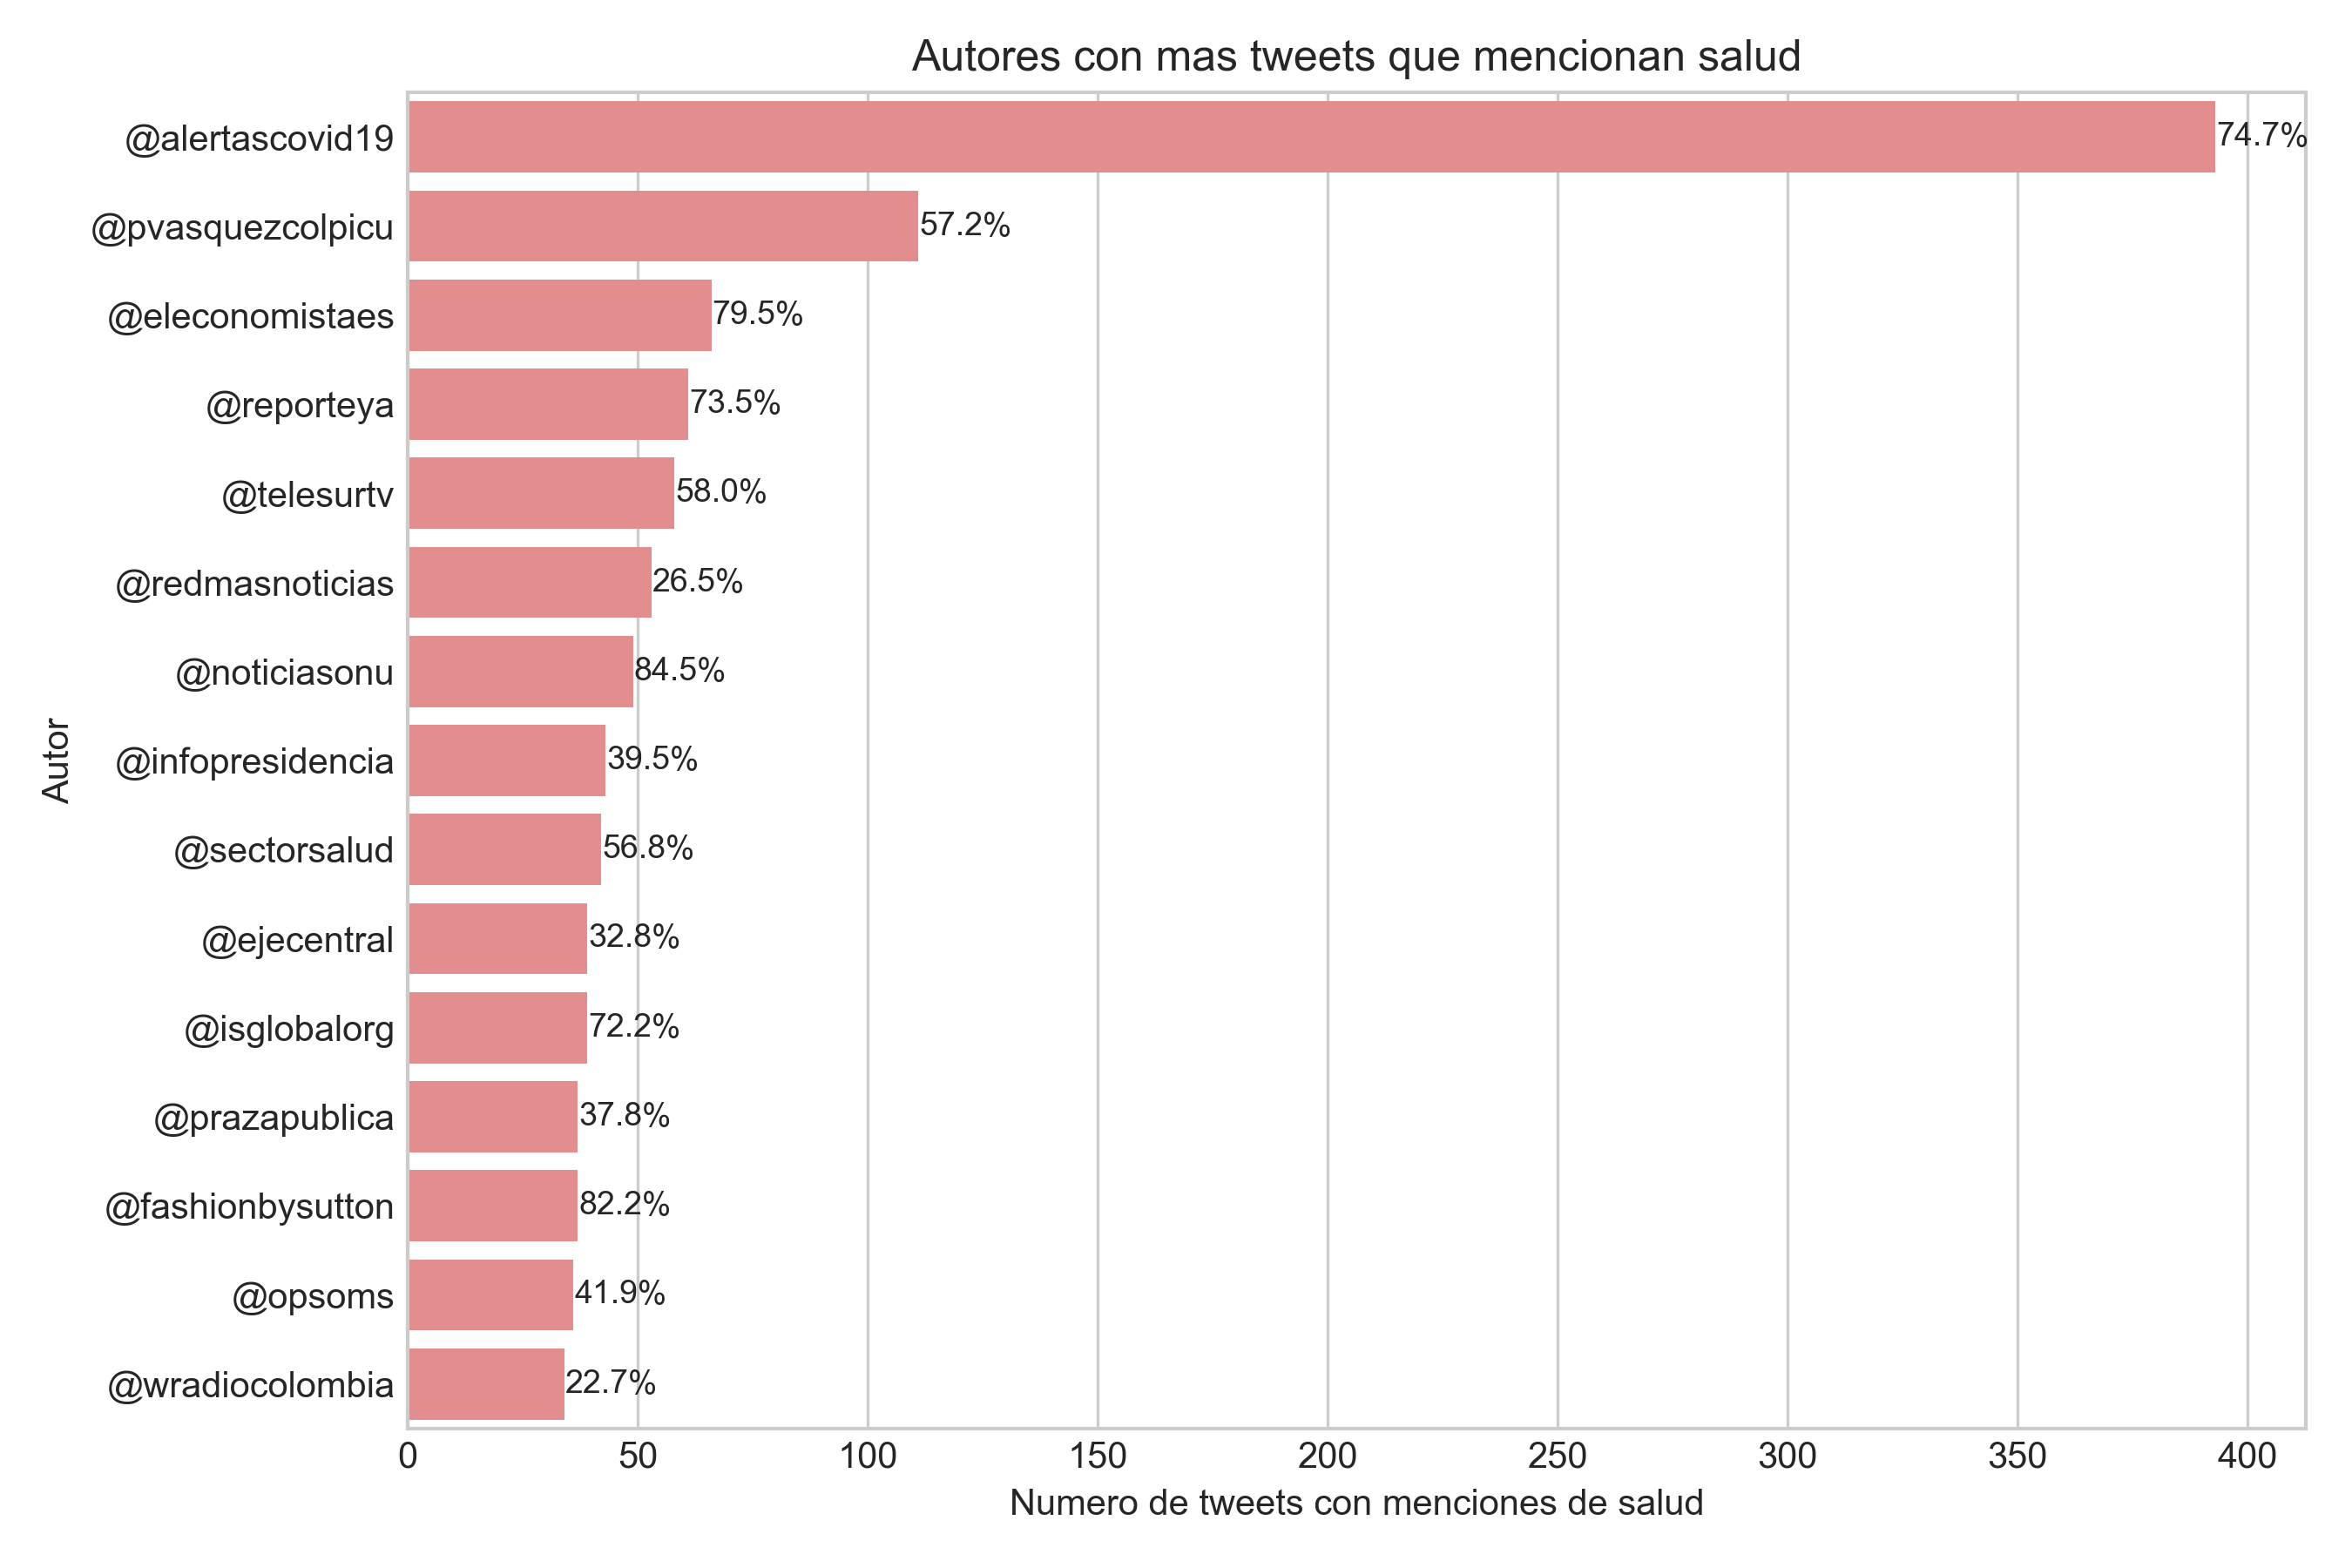
\includegraphics[width=\linewidth]{fig_autores_salud_simple.png}
        \caption*{\small Top 15 autores por n\'umero de tweets de salud}
      \end{figure}

    \column{0.5\textwidth}
      \begin{figure}
        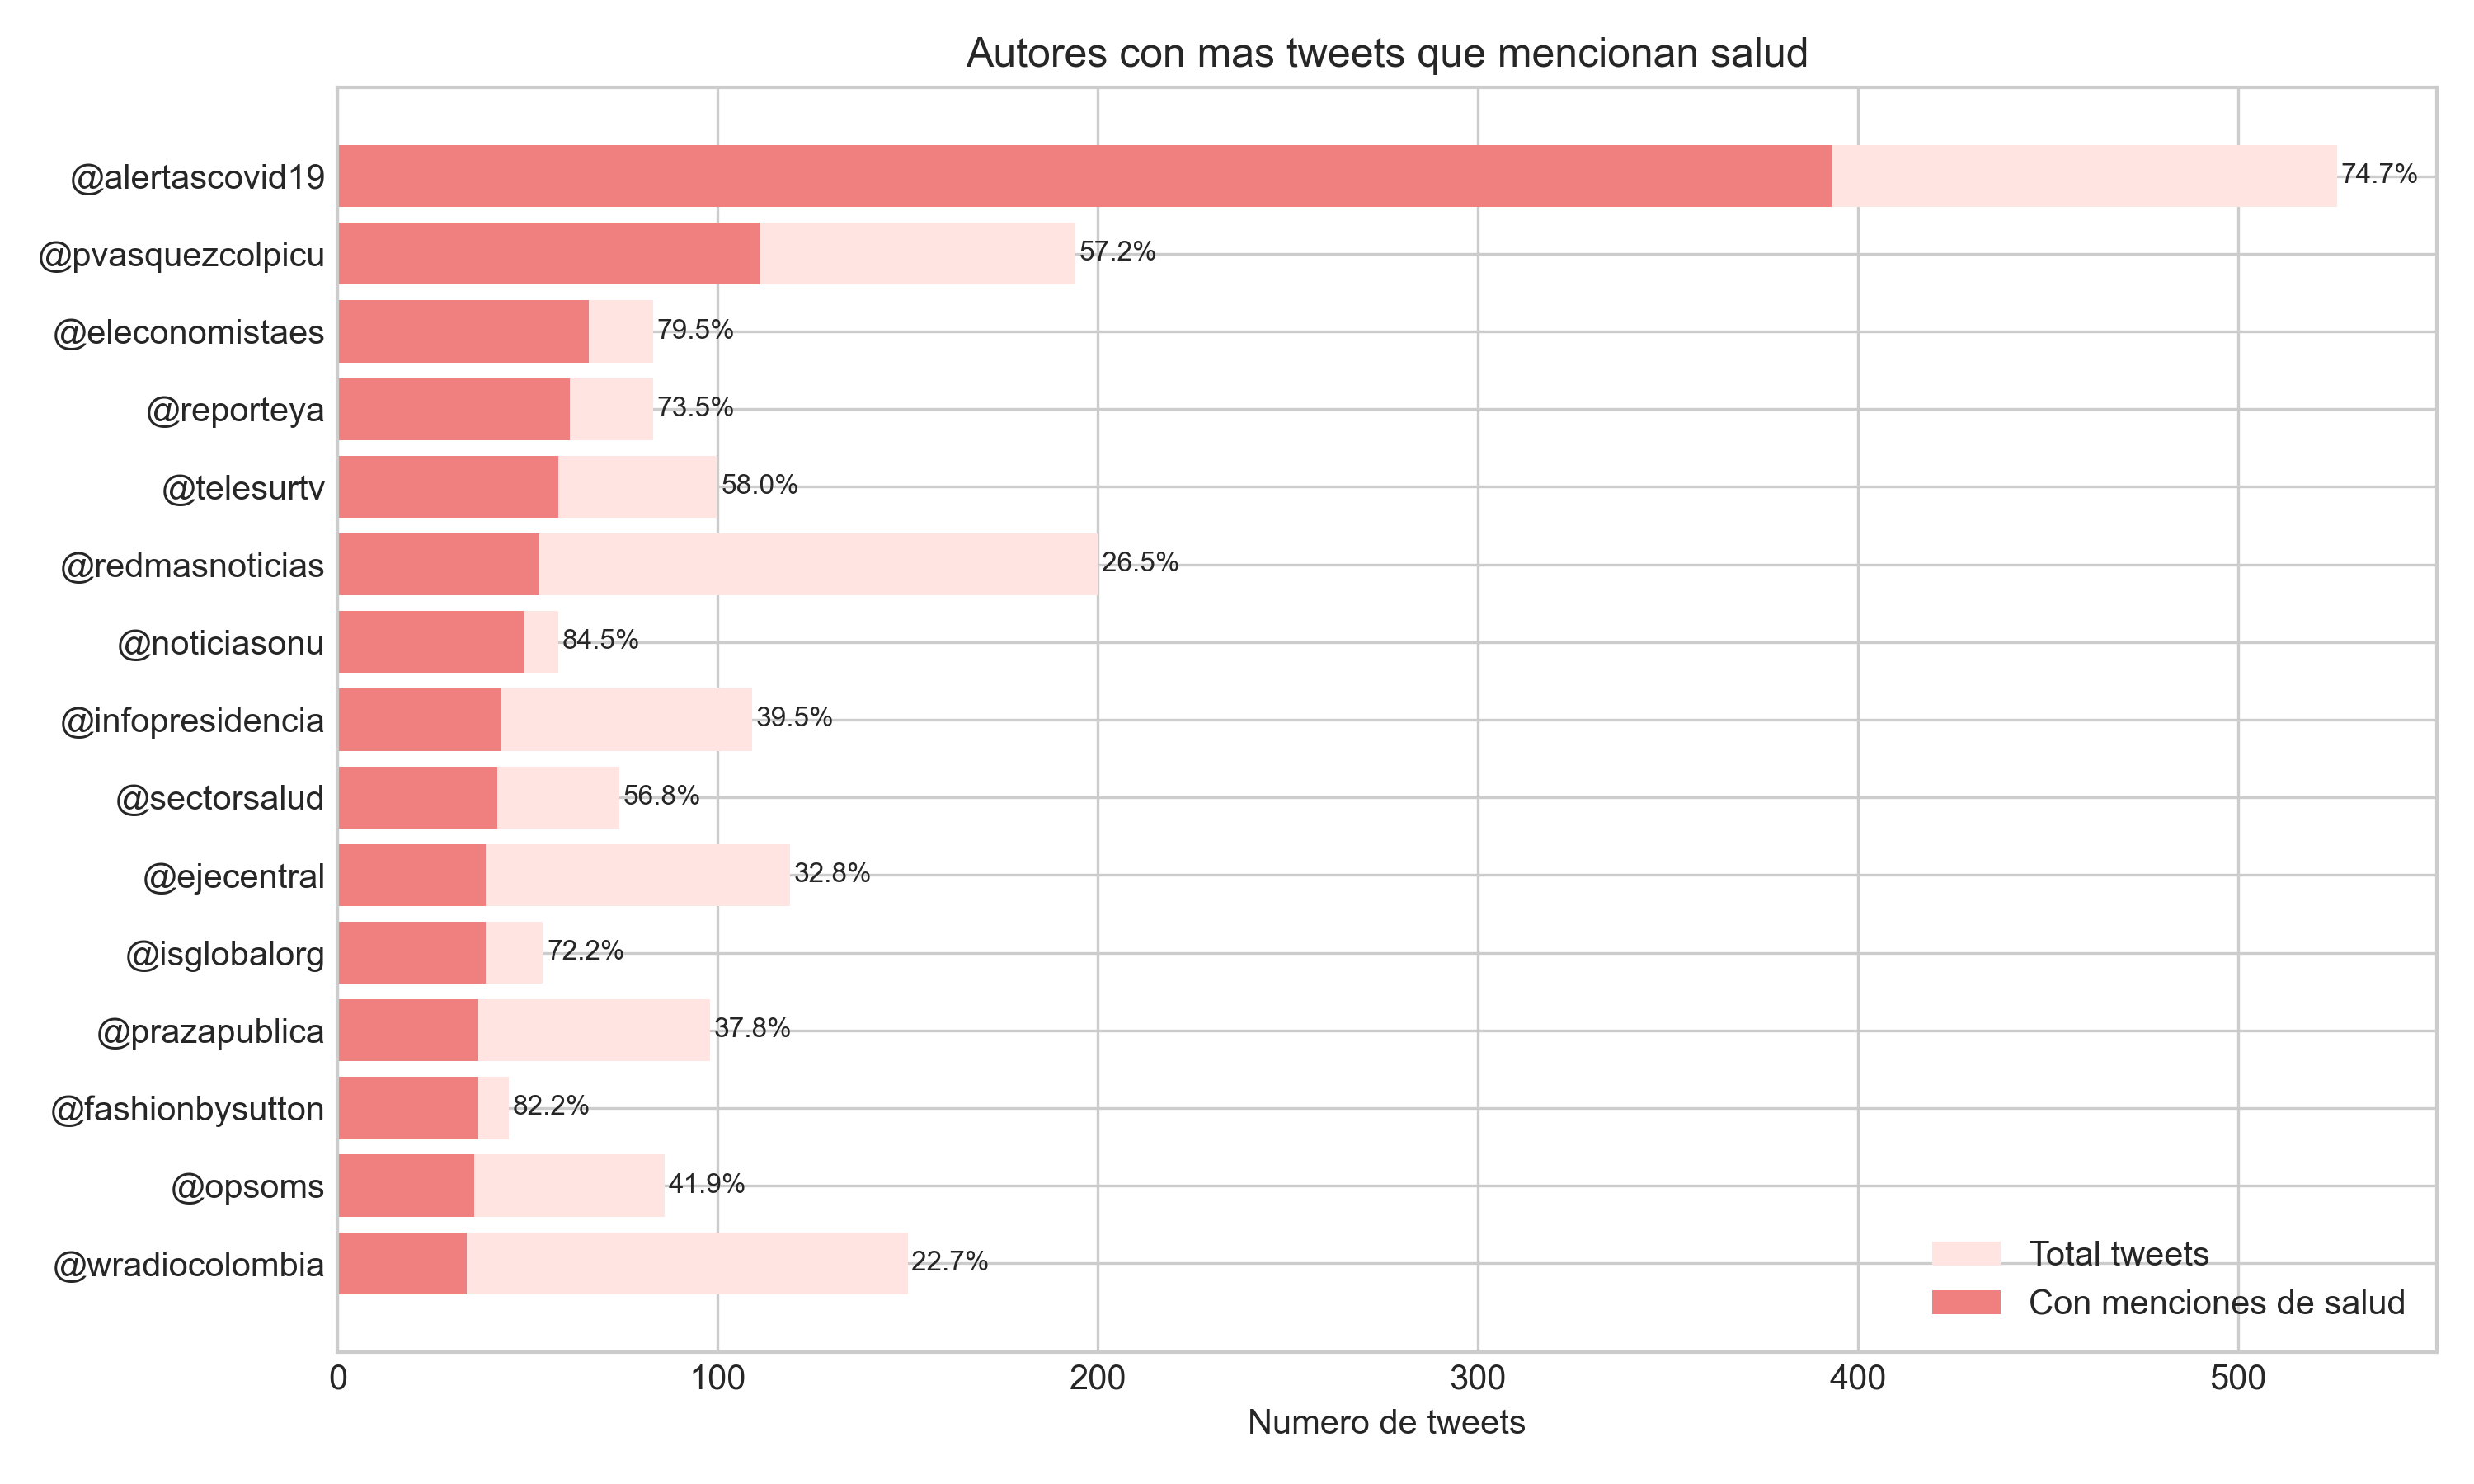
\includegraphics[width=\linewidth]{fig_autores_salud_comparativo.png}
        \caption*{\small Tweets de salud vs.\ total de tweets, mismos autores}
      \end{figure}
  \end{columns}

  \medskip
  \begin{itemize}
    \item Los porcentajes muestran qu\'e proporci\'on del
          total de tweets de cada autor corresponde a salud.
    \item Algunos autores tienen un volumen alto en
          t\'erminos absolutos pero una proporci\'on baja,
          y viceversa.
  \end{itemize}

\end{frame}

% ---------------------------------------------------
% Diapositiva 7: Top autores (avanzado) y tipo de cuenta
\begin{frame}{Top autores y tipo de cuenta}

  \begin{columns}[T]
    \column{0.5\textwidth}
      \begin{figure}
        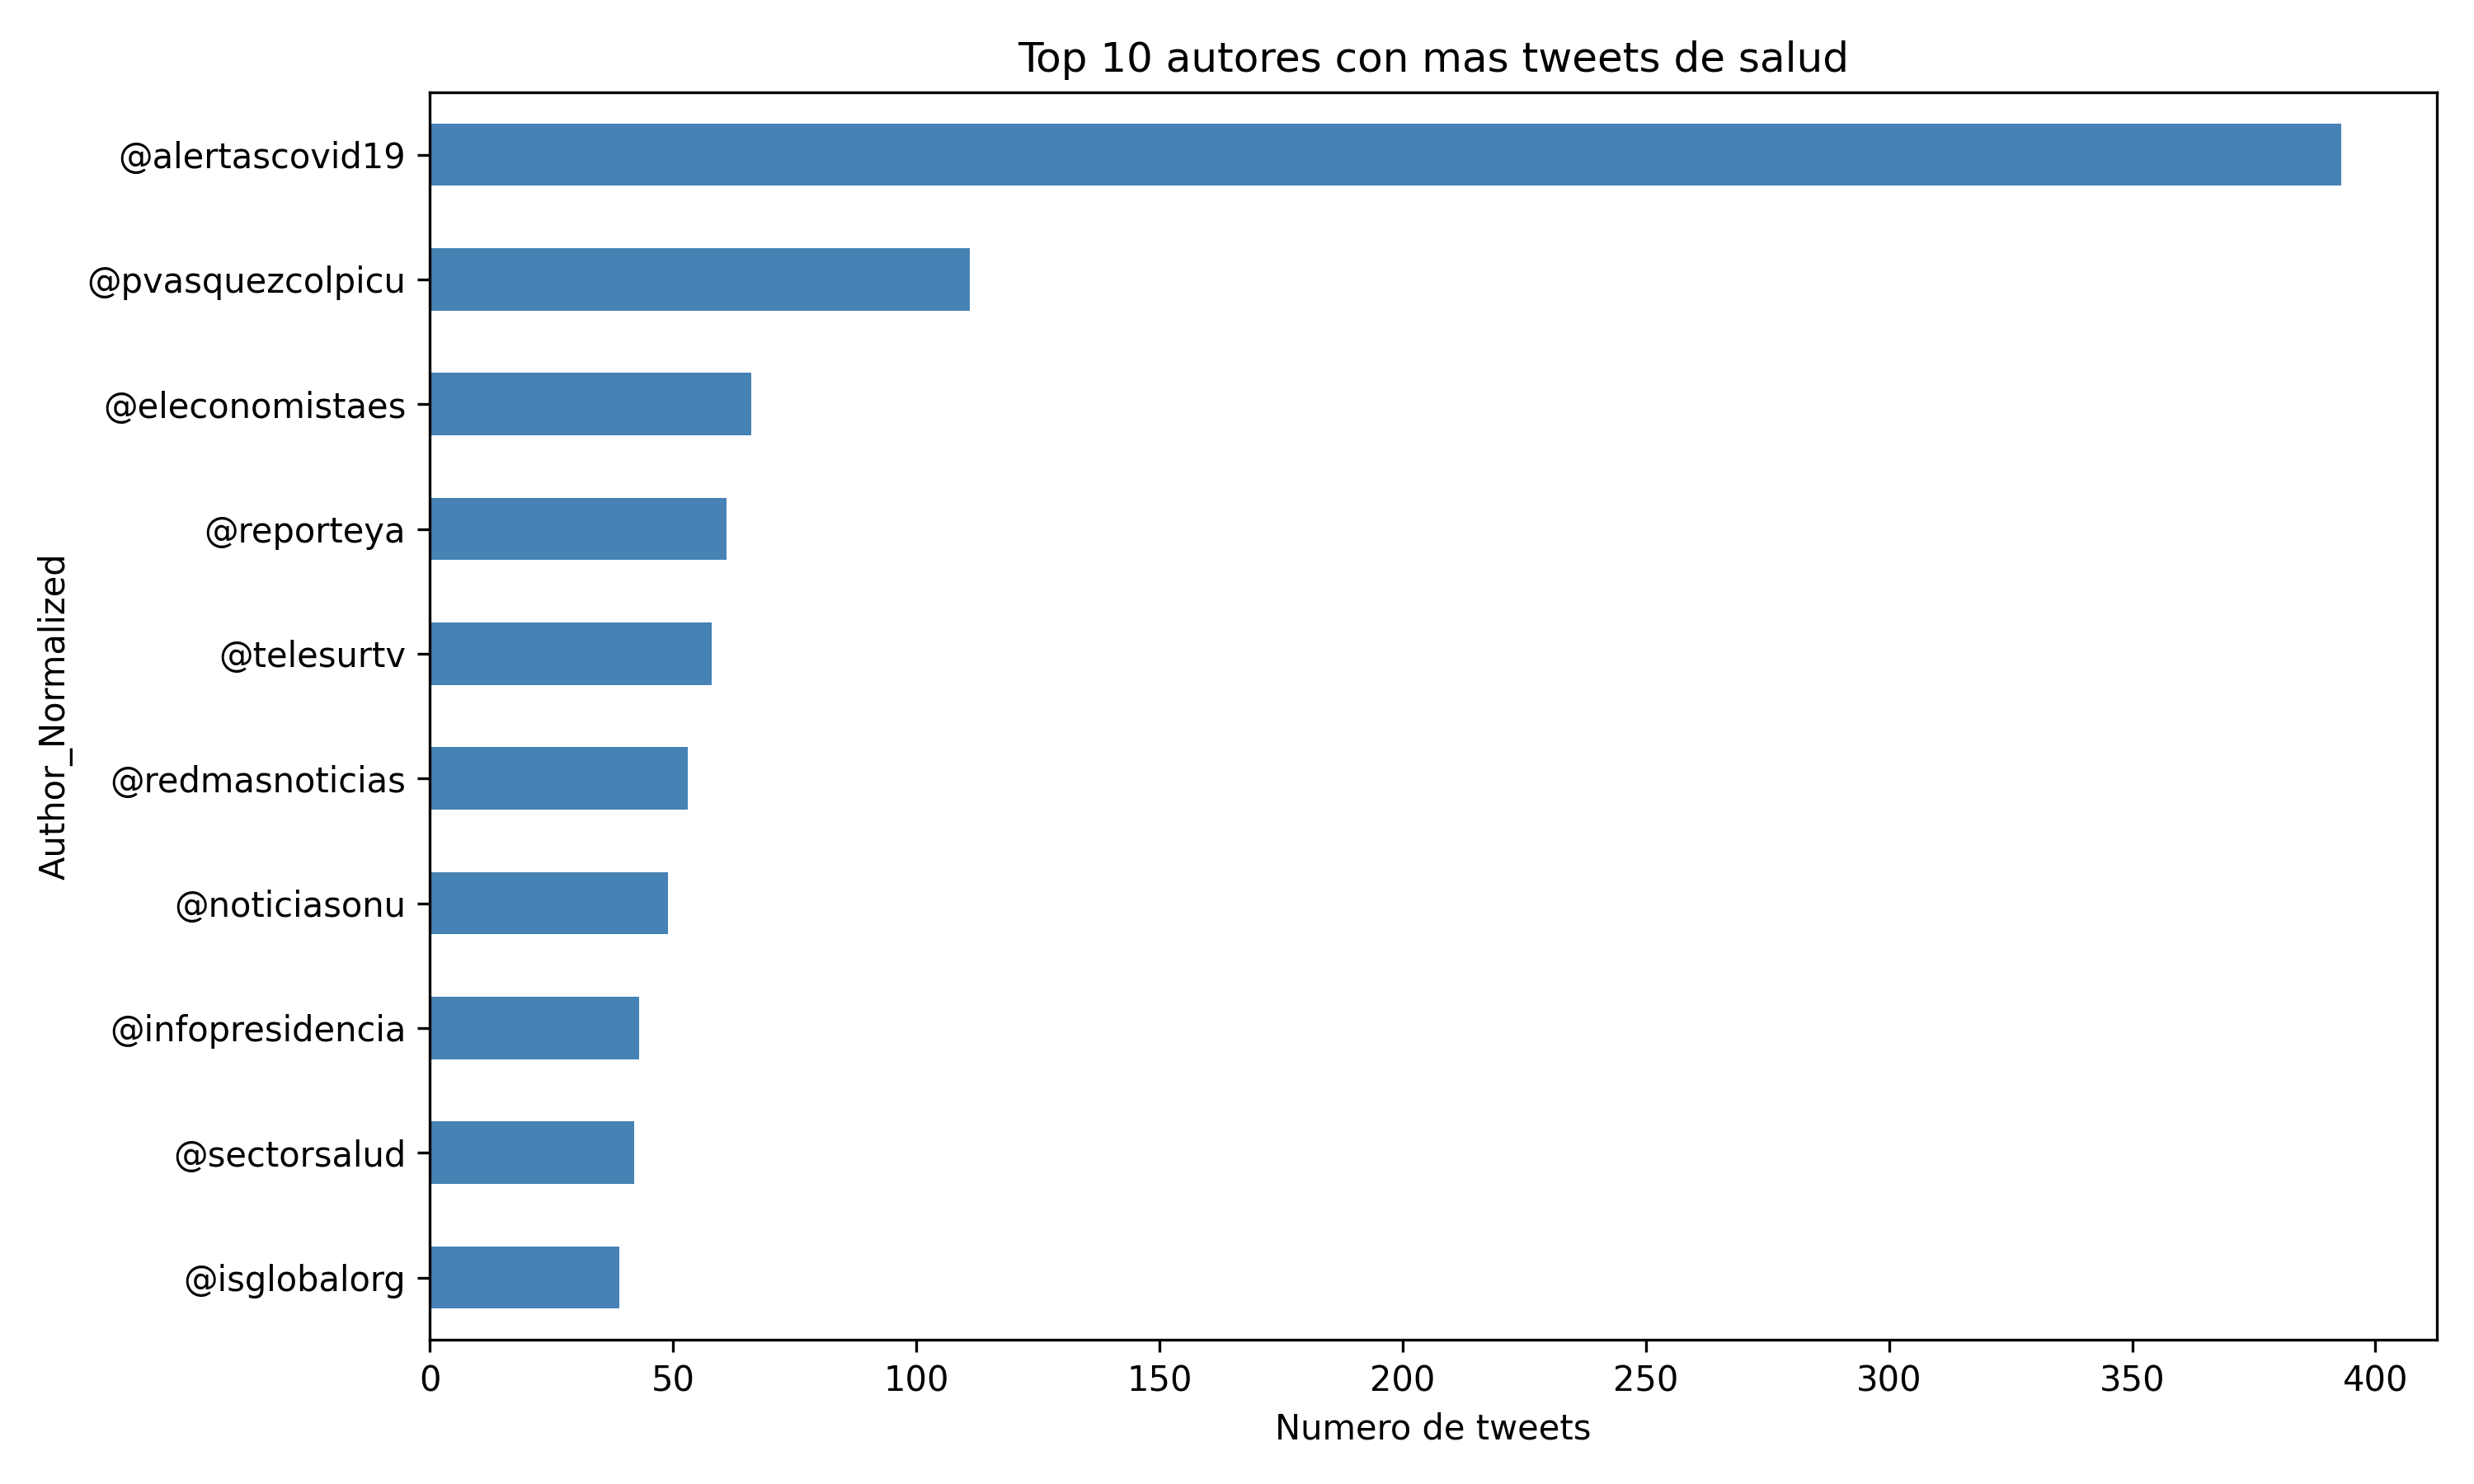
\includegraphics[width=\linewidth]{fig_top_autores_salud_avanzado.png}
        \caption*{\small Top 10 autores con m\'as tweets de salud}
      \end{figure}

    \column{0.5\textwidth}
      \begin{figure}
        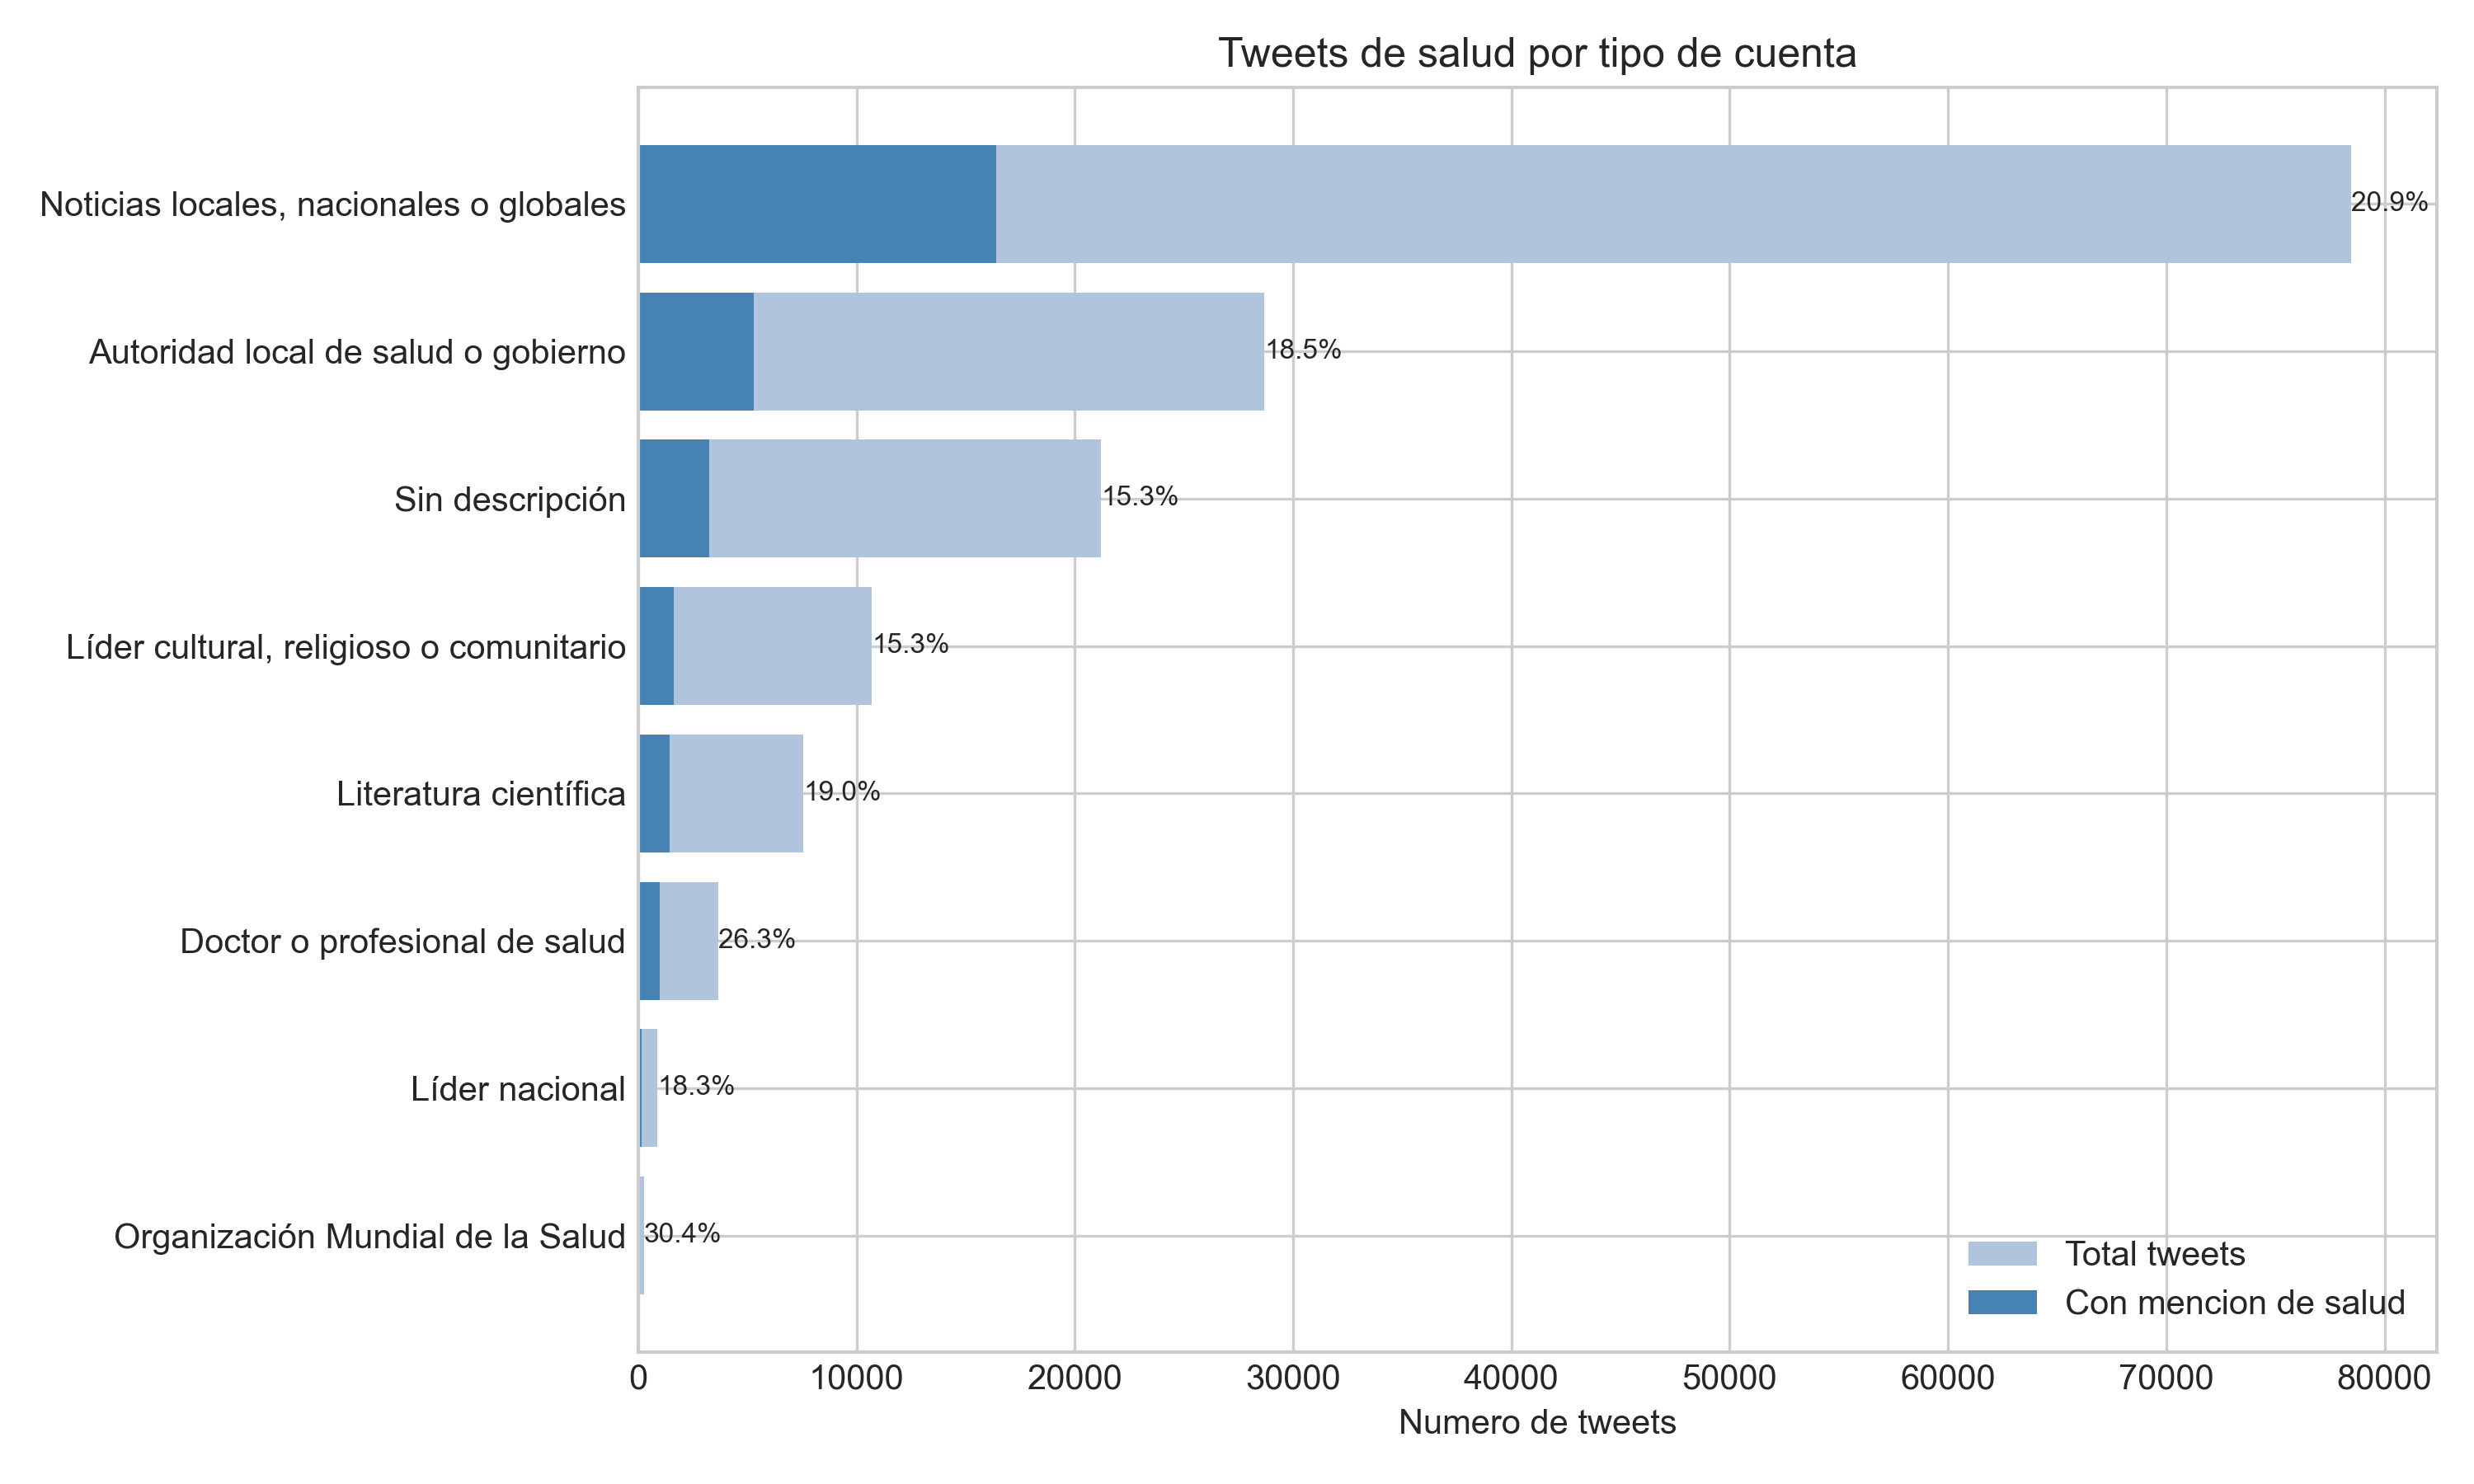
\includegraphics[width=\linewidth]{fig_entidad_salud.png}
        \caption*{\small Tweets de salud por tipo de cuenta (entidad)}
      \end{figure}
  \end{columns}

  \medskip
  \begin{itemize}
    \item Permite identificar qu\'e tipos de cuenta
          (medios, instituciones, personas, etc.)
          concentran las menciones de salud.
  \end{itemize}

\end{frame}

% ---------------------------------------------------
% Diapositiva 8: Figuras clave e instituciones
\begin{frame}{Figuras clave e instituciones de salud}

  \begin{columns}[T]
    \column{0.5\textwidth}
      \begin{figure}
        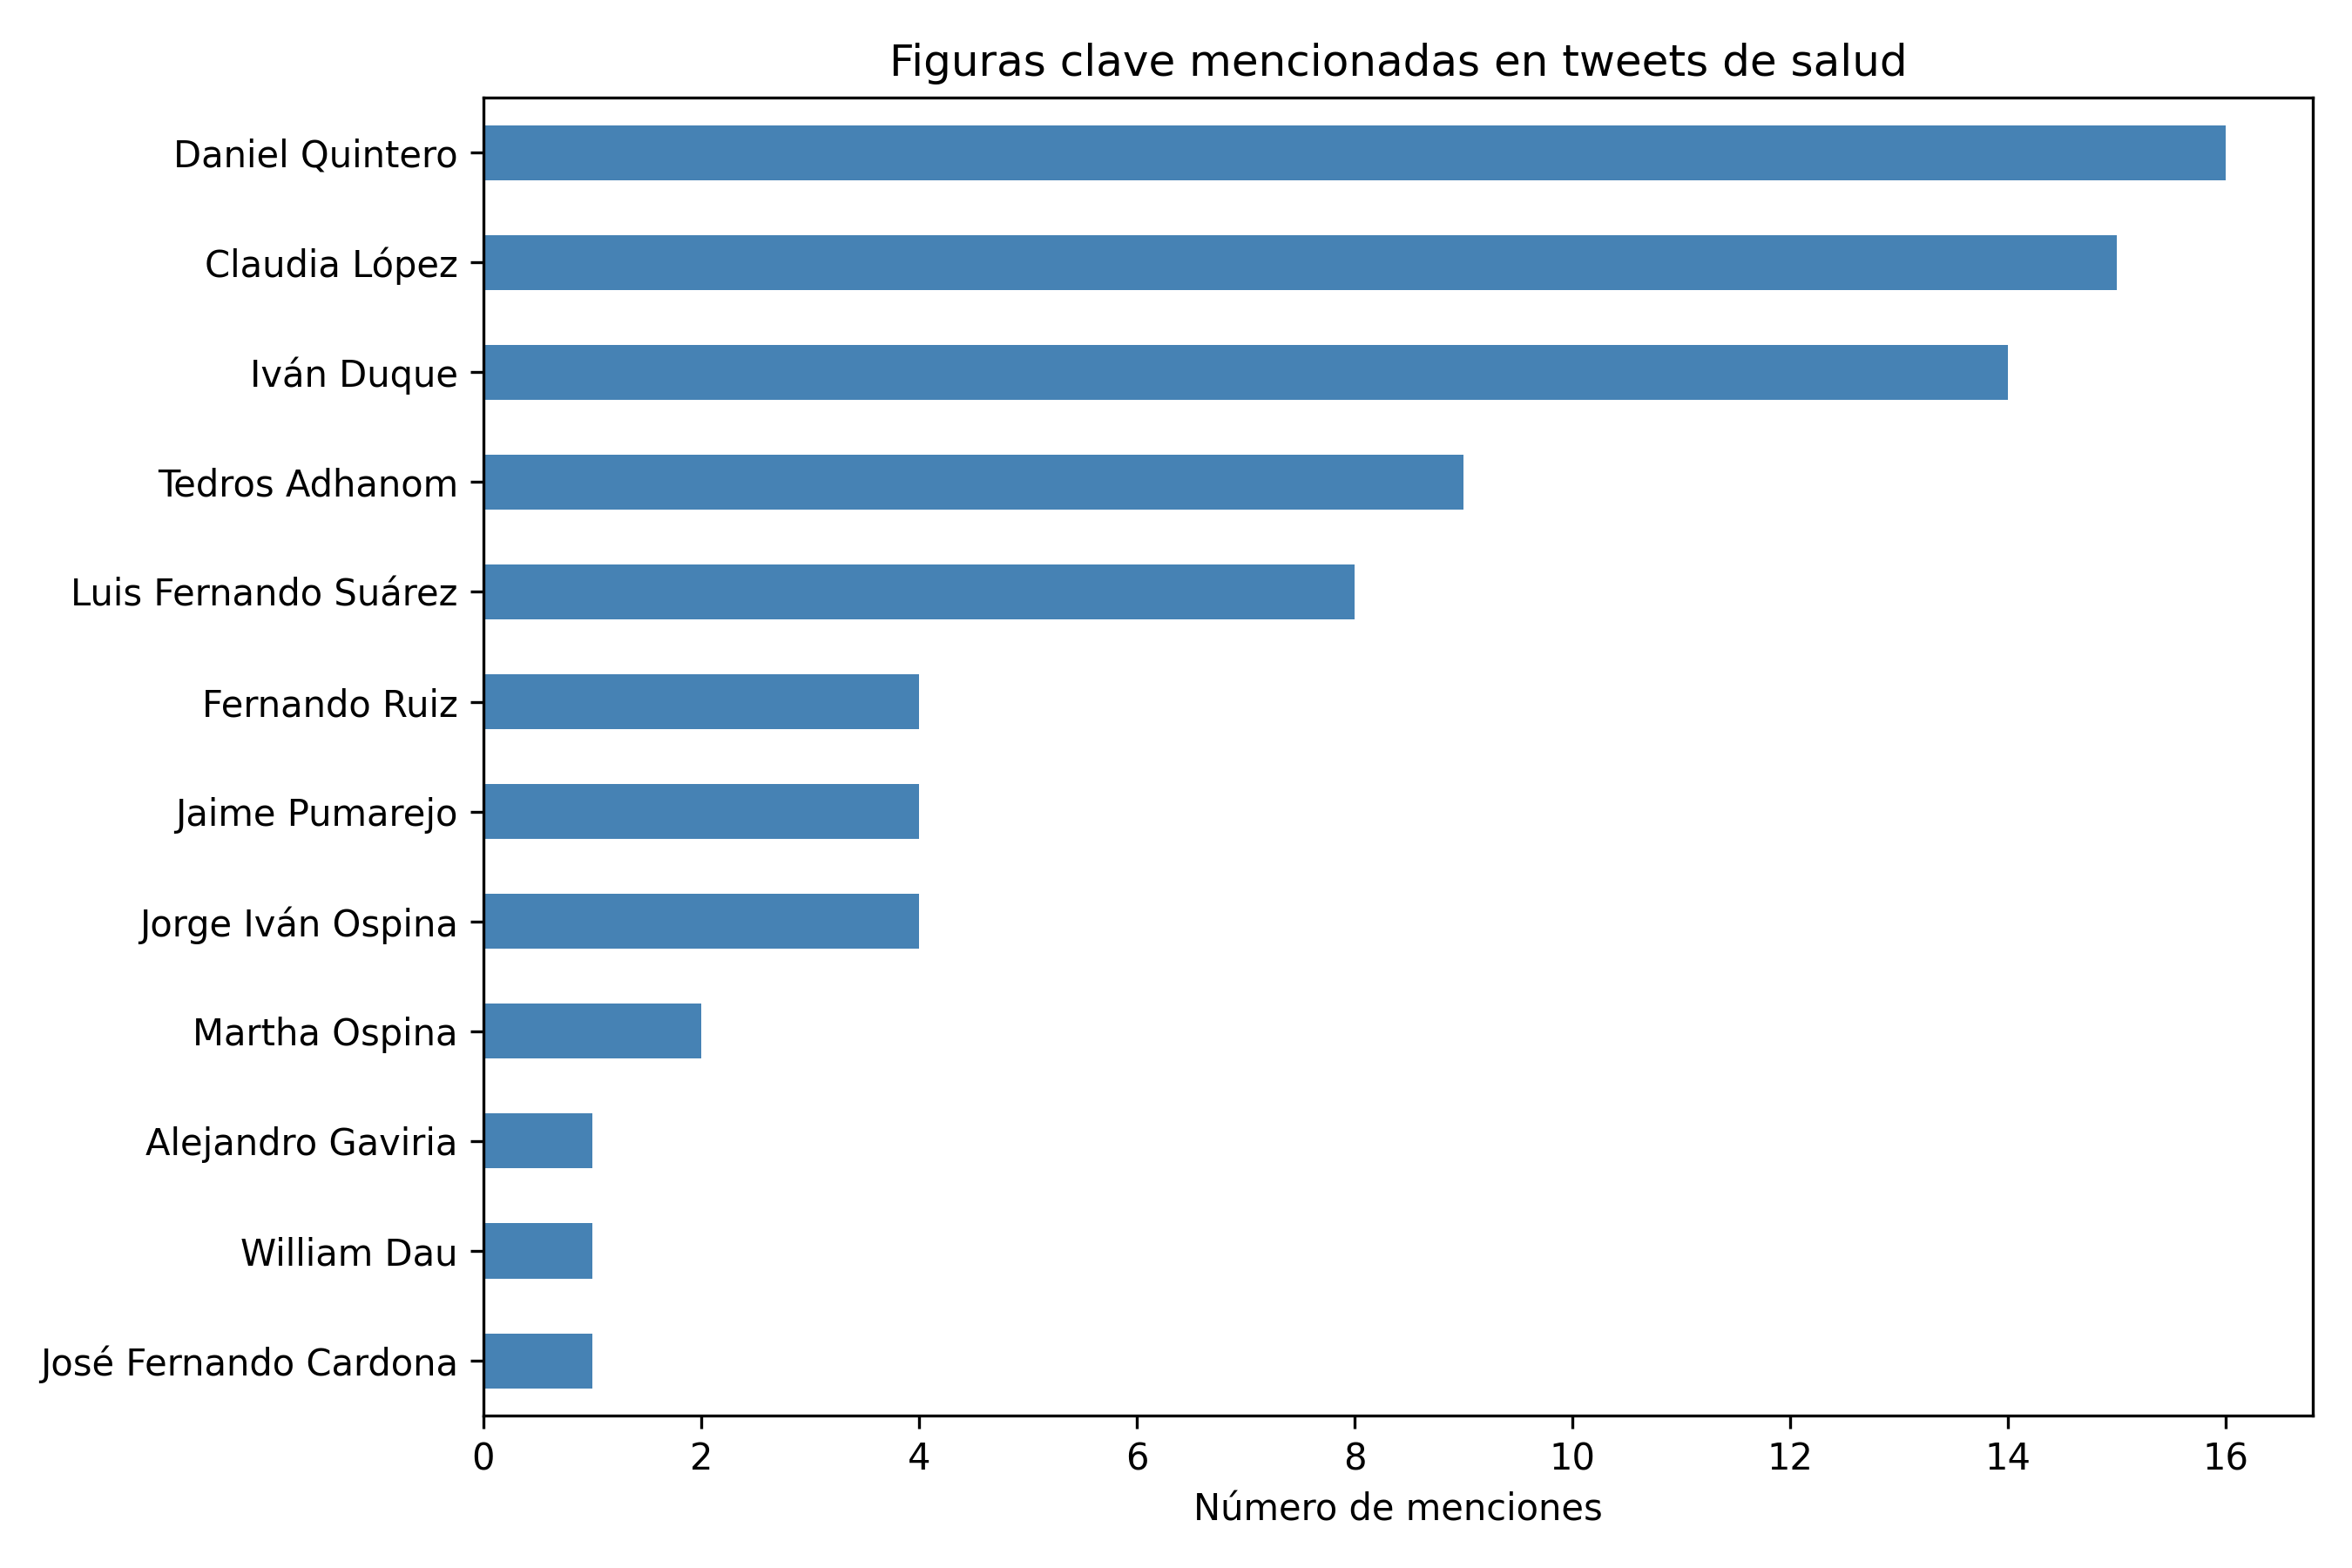
\includegraphics[width=\linewidth]{fig_top_autores_salud_busqueda.png}
        \caption*{\small Figuras clave mencionadas en tweets de salud}
      \end{figure}

    \column{0.5\textwidth}
      \begin{figure}
        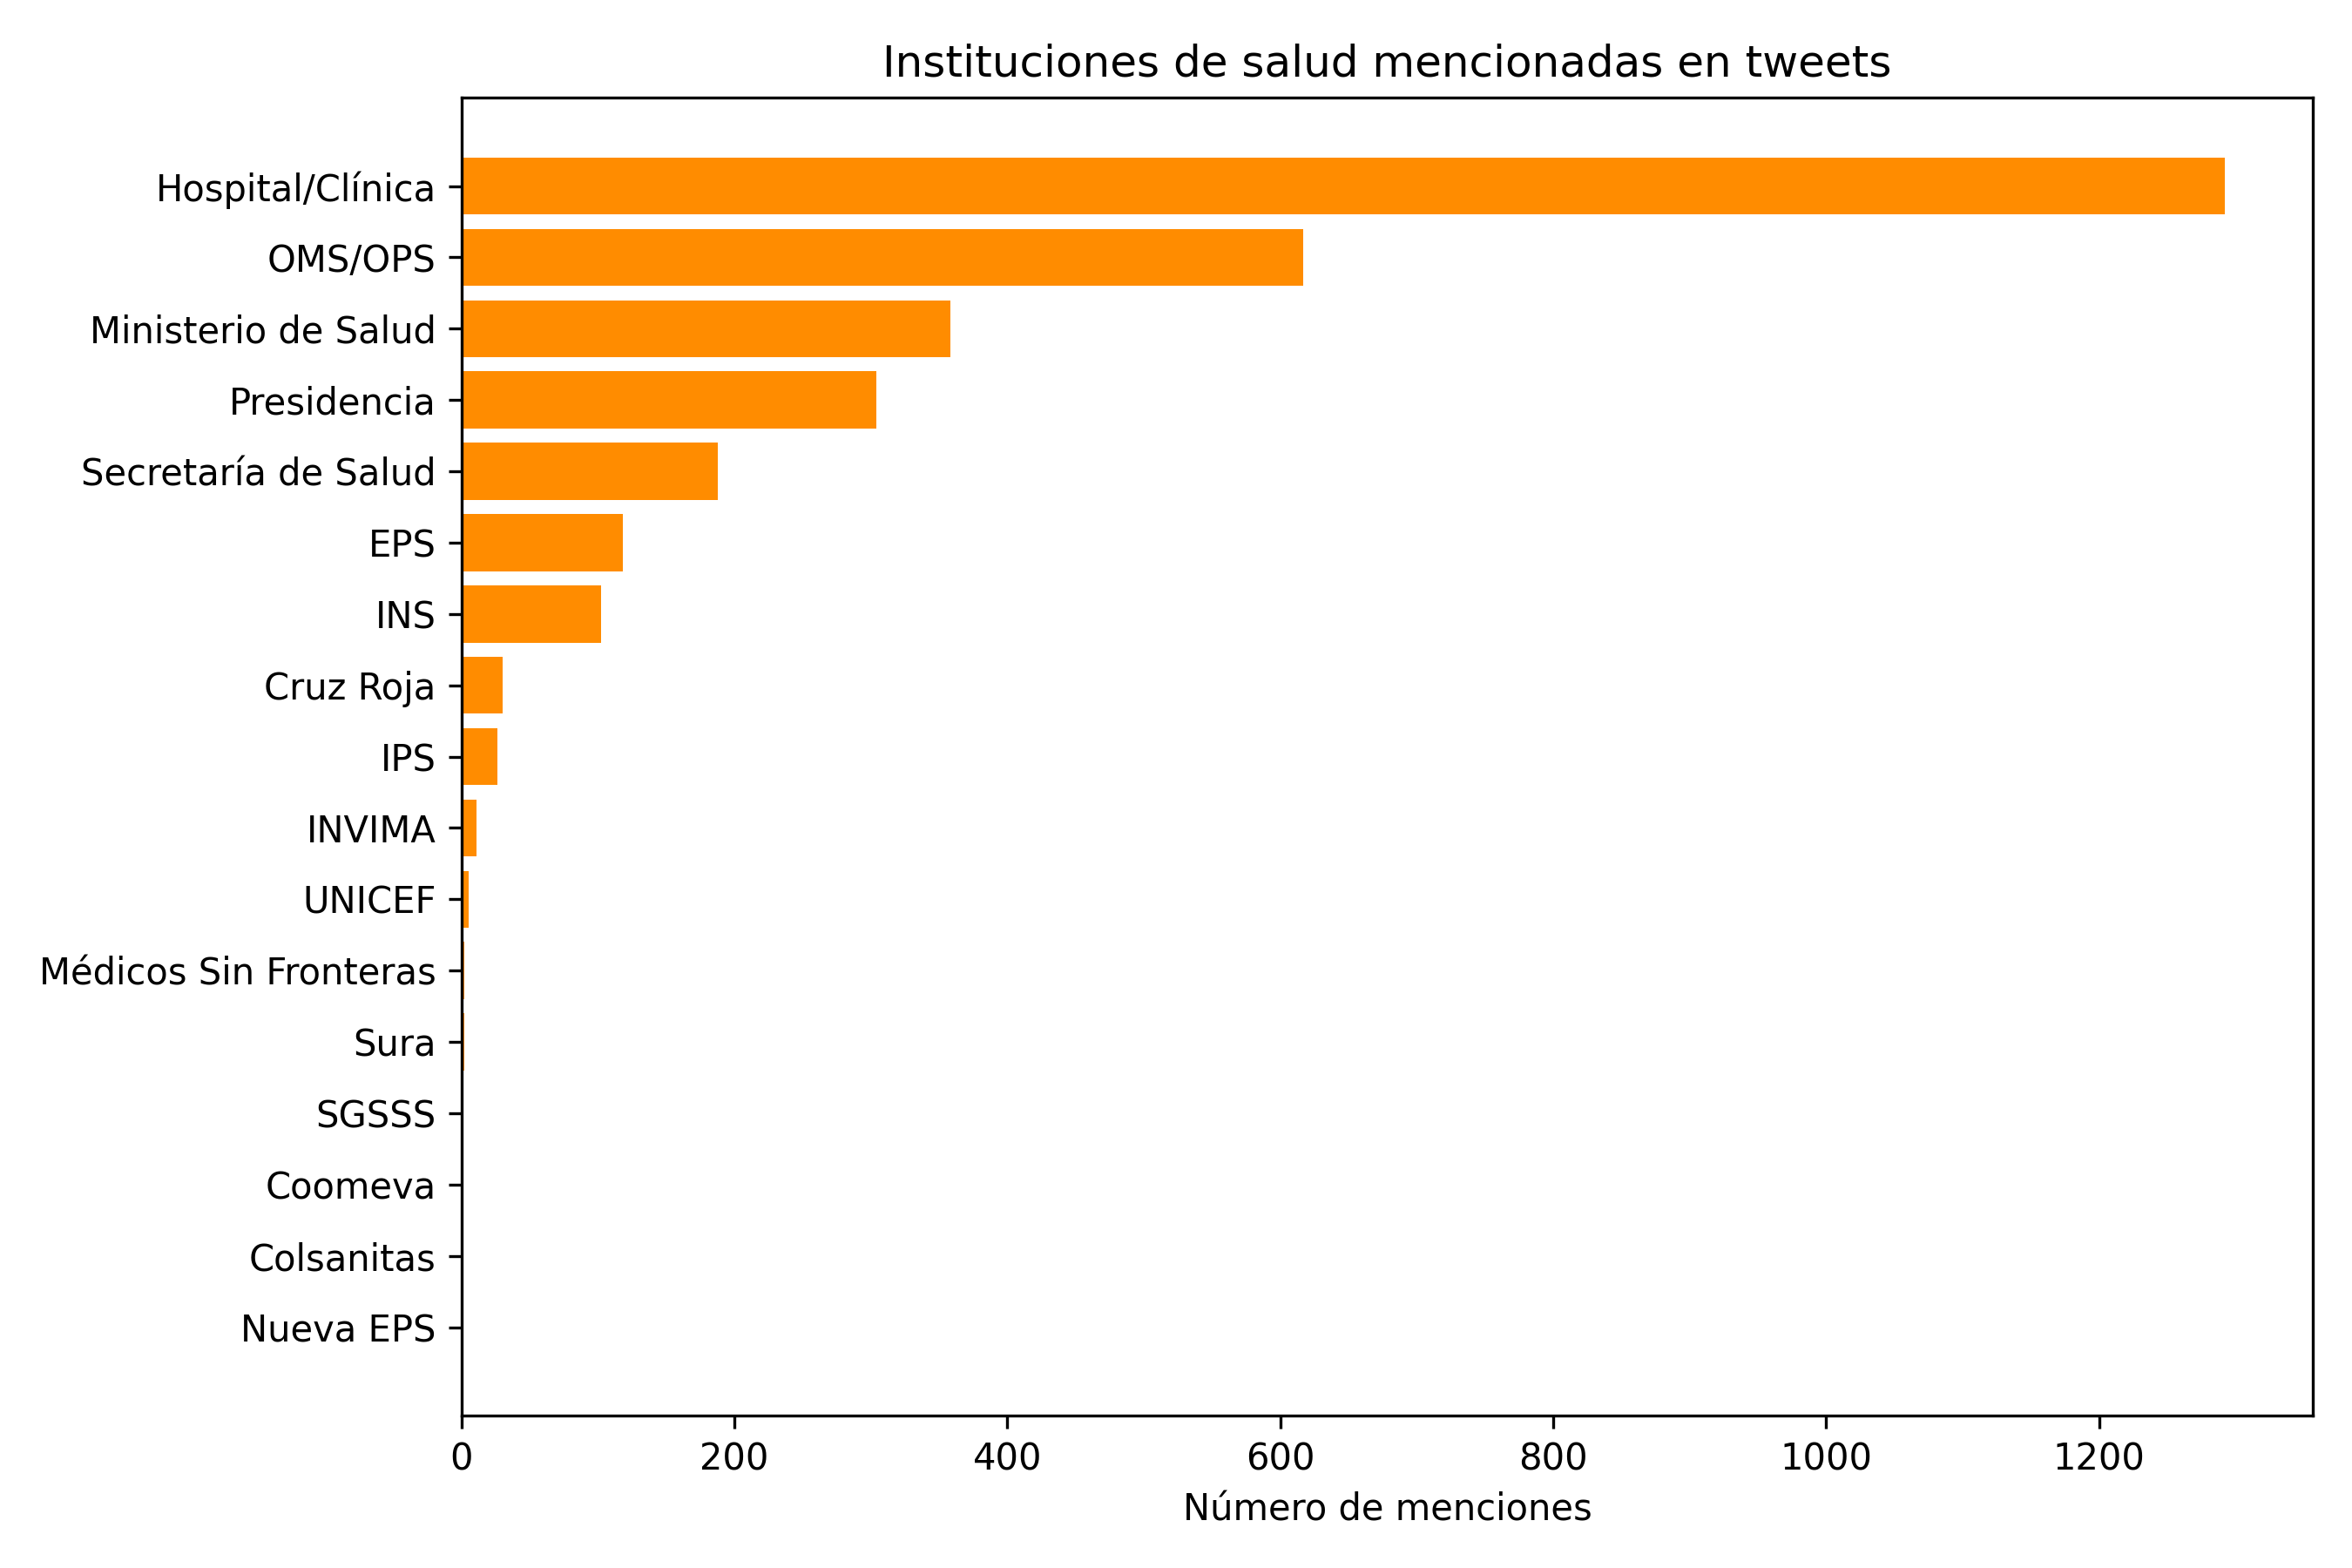
\includegraphics[width=\linewidth]{fig_top_instituciones_salud.png}
        \caption*{\small Instituciones de salud mencionadas}
      \end{figure}
  \end{columns}

  \medskip
  \begin{itemize}
    \item B\'usqueda dirigida (por diccionarios/regex) de
          personajes p\'ublicos e instituciones de salud
          colombianas e internacionales.
  \end{itemize}

\end{frame}

% ---------------------------------------------------
% Diapositiva 9: Departamentos
\begin{frame}{Geograf\'ia de las menciones de salud}

  \begin{figure}
    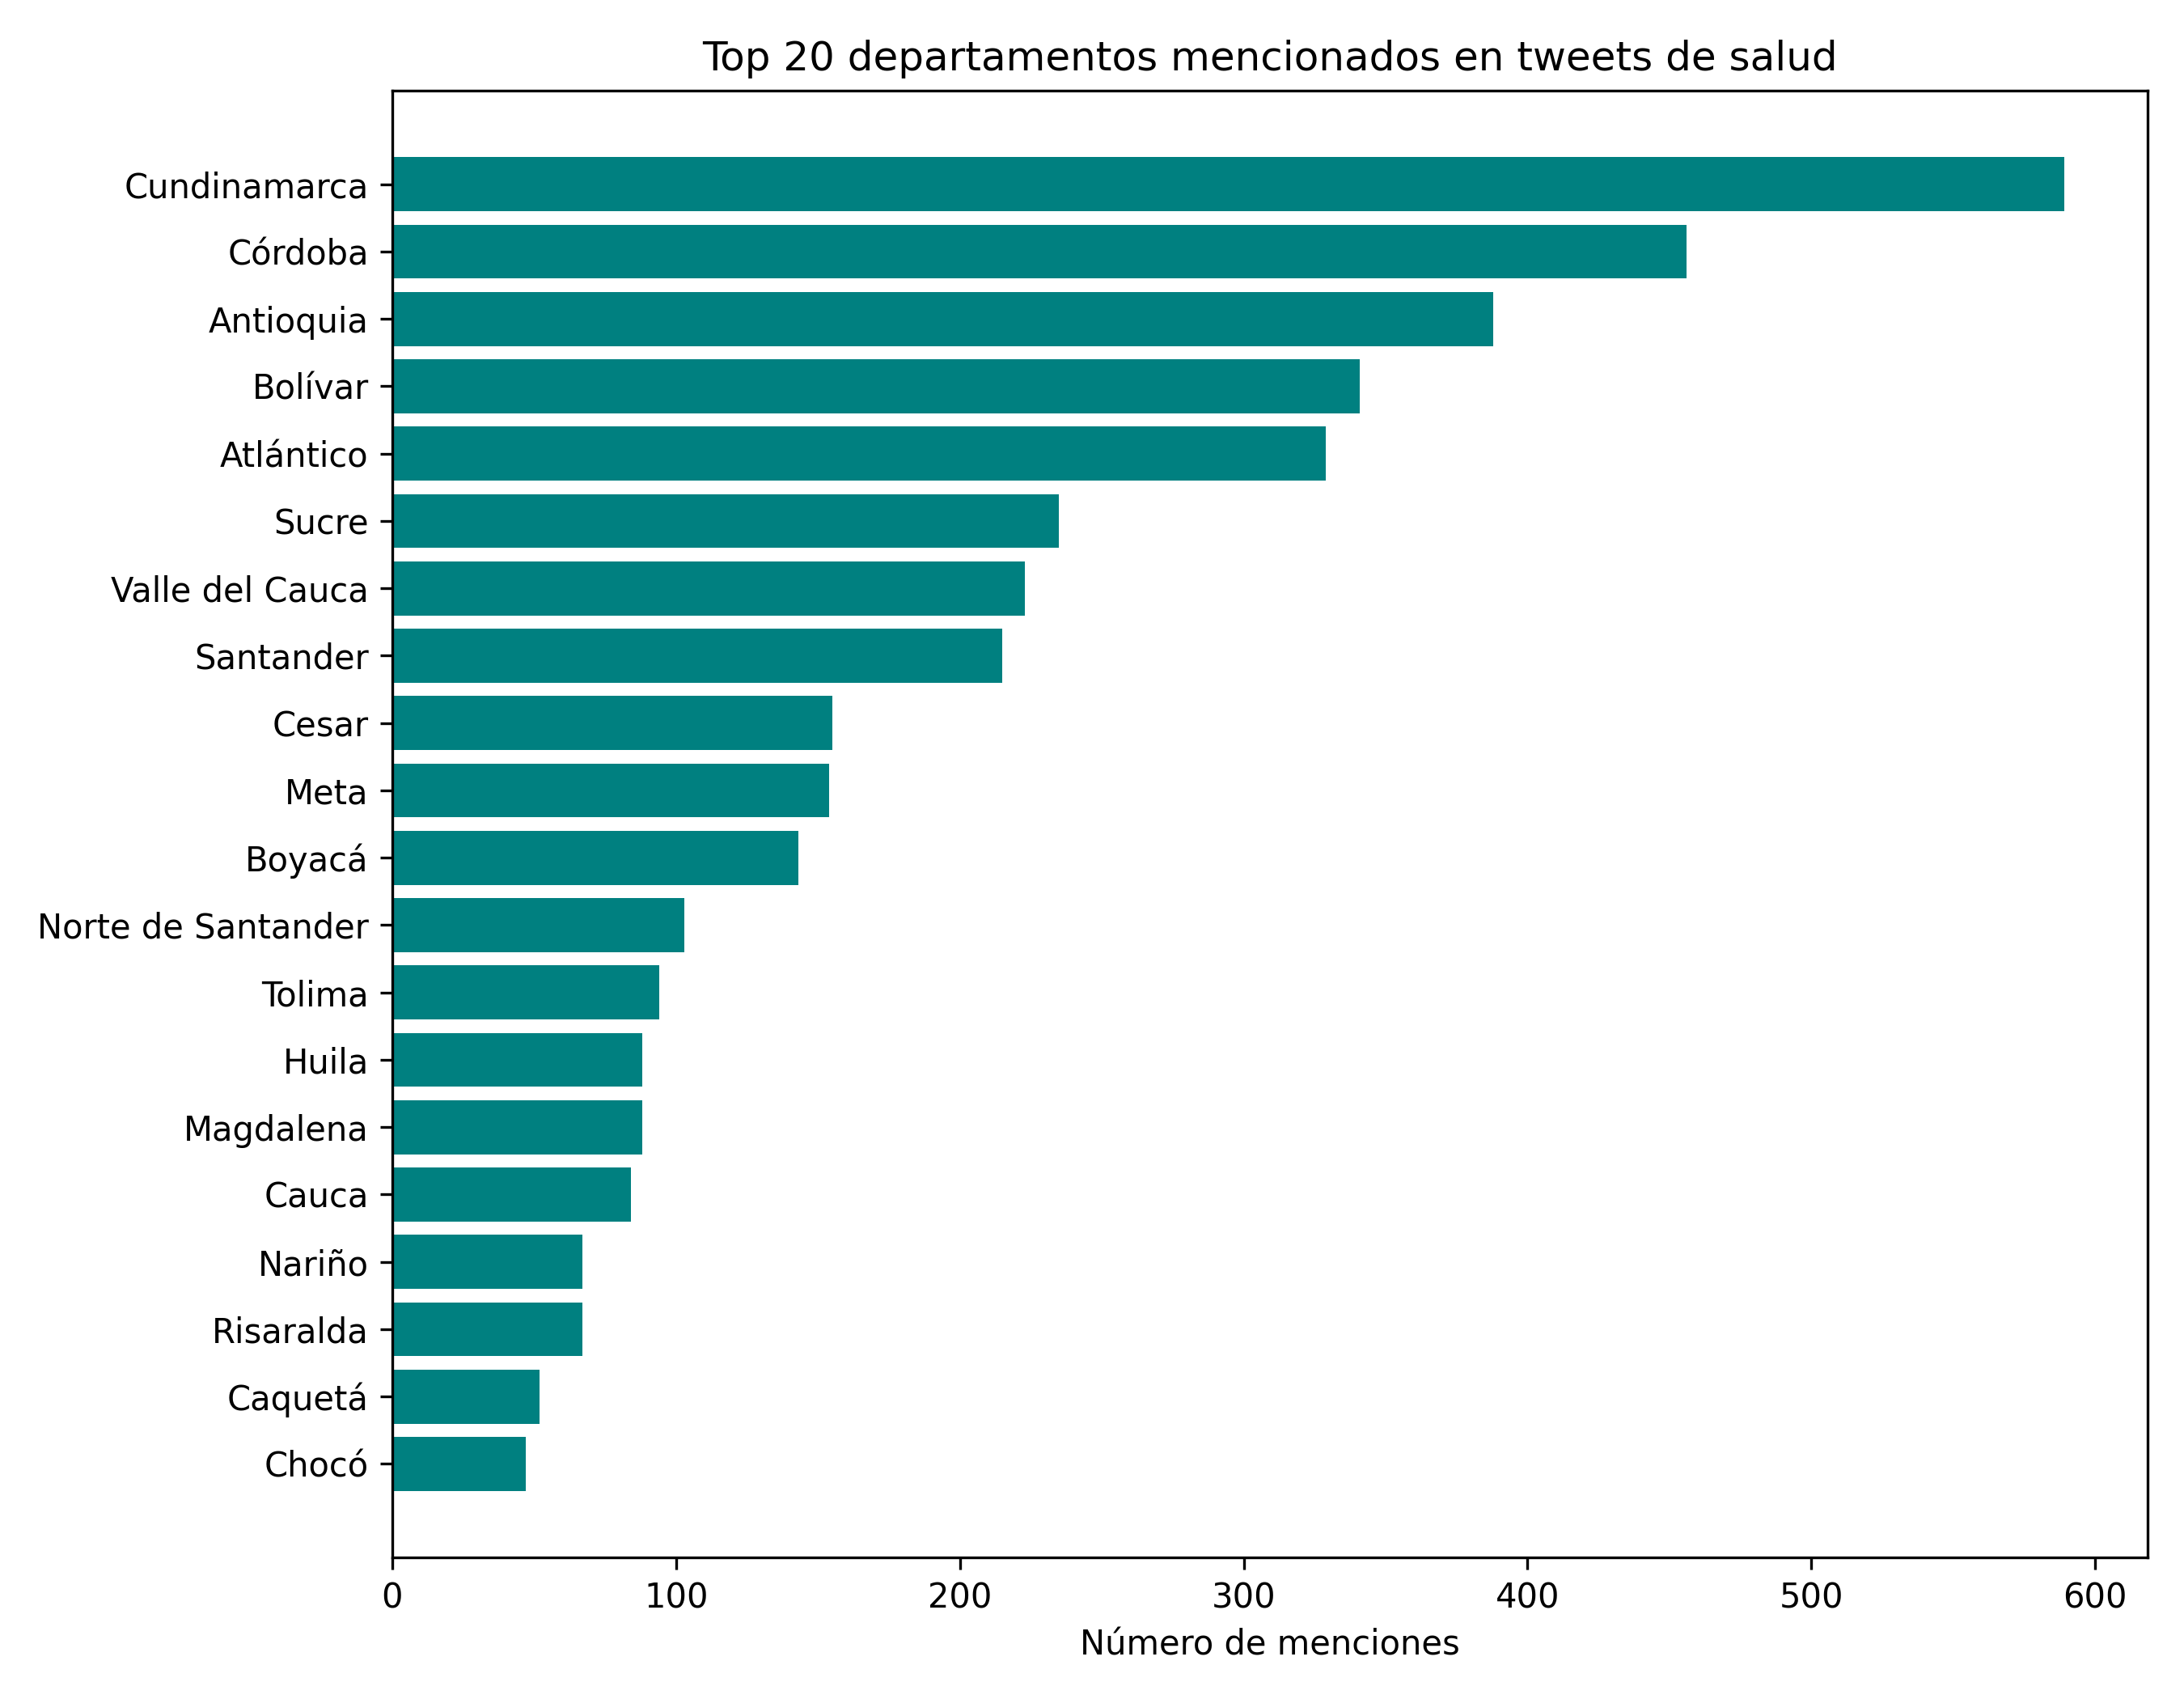
\includegraphics[width=0.7\linewidth]{fig_top_departamentos_salud.png}
  \end{figure}

  \begin{center}
  \small
  Top 20 departamentos colombianos (y ciudades principales)
  mencionados en tweets que hablan de salud.
  \end{center}

\end{frame}

% ---------------------------------------------------
% Diapositiva 10: Nubes de palabras
\begin{frame}{Nubes de palabras del subcorpus de salud}

  \begin{columns}[T]
    \column{0.5\textwidth}
      \begin{figure}
        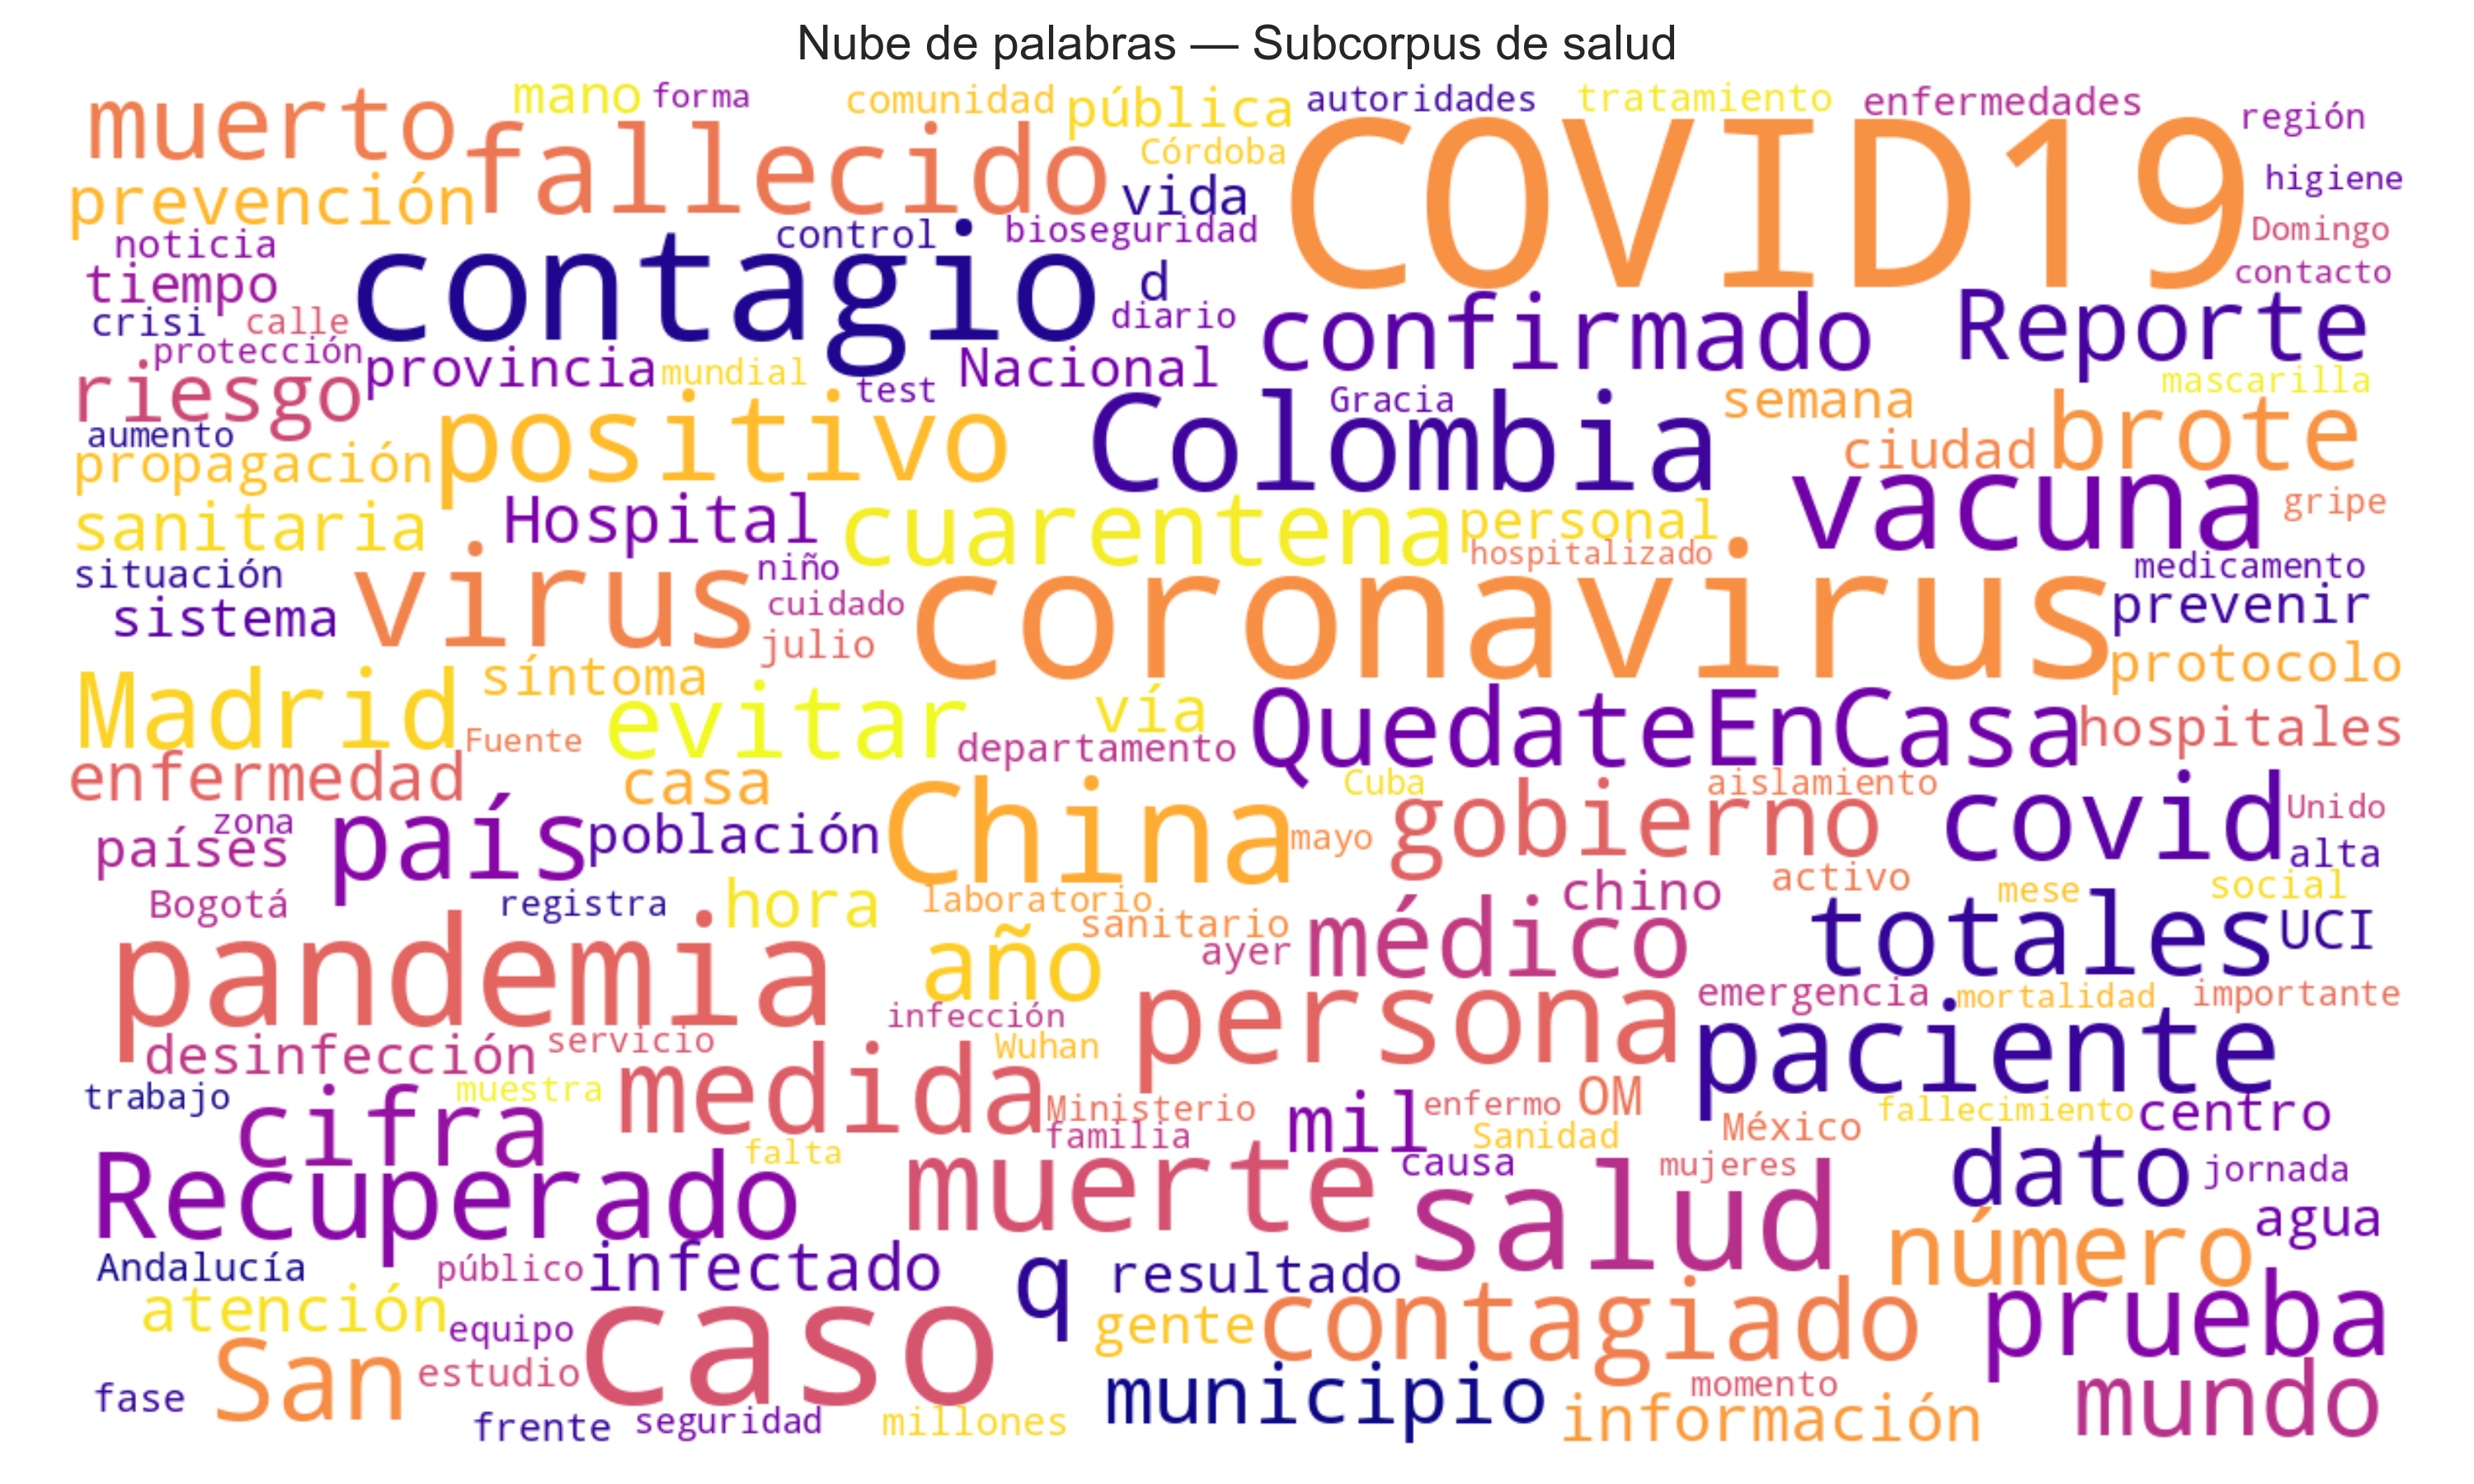
\includegraphics[width=\linewidth]{nube_subcorpus_salud.png}
      \end{figure}

    \column{0.5\textwidth}
      \begin{figure}
        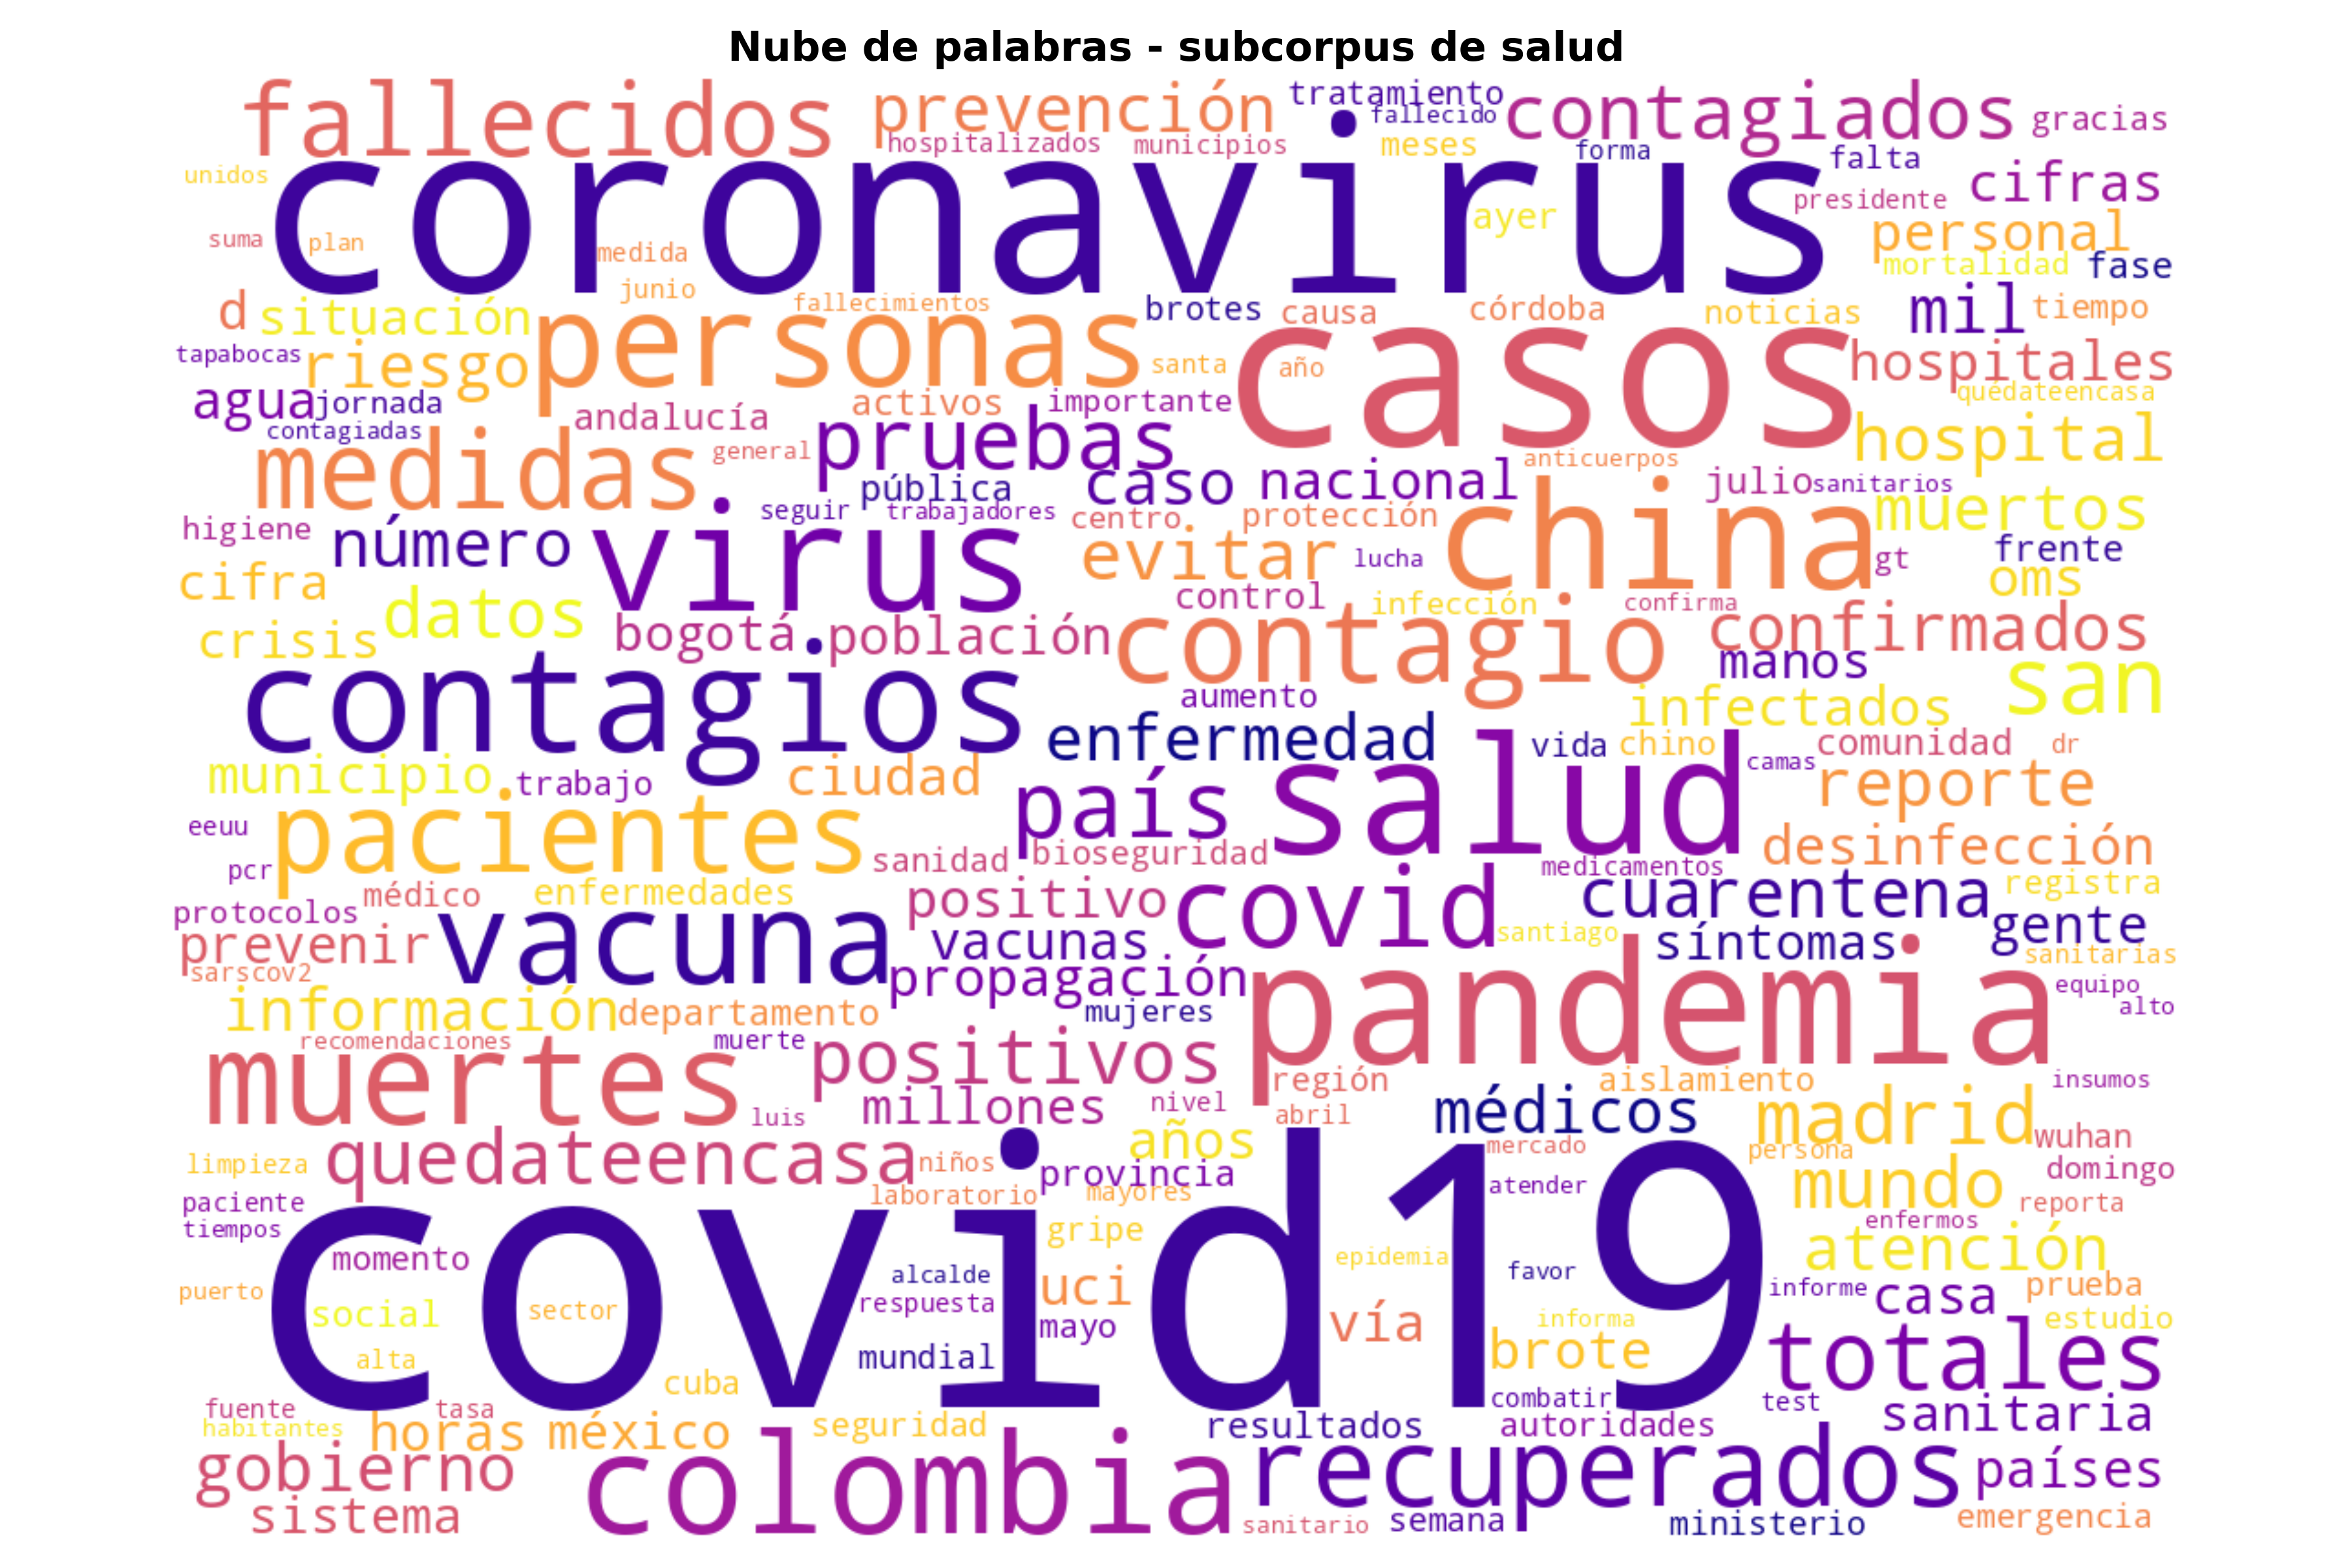
\includegraphics[width=\linewidth]{nube_subcorpus_salud_avanzado.png}
      \end{figure}
  \end{columns}

  \begin{center}
  \small
  Palabras m\'as frecuentes (lematizadas, sin palabras vac\'ias)
  en los tweets que mencionan temas de salud.
  \end{center}

\end{frame}

% ---------------------------------------------------
% Diapositiva 11: Frecuencias POS
\begin{frame}{Frecuencias gramaticales (POS) en el subcorpus de salud}

  \begin{figure}
    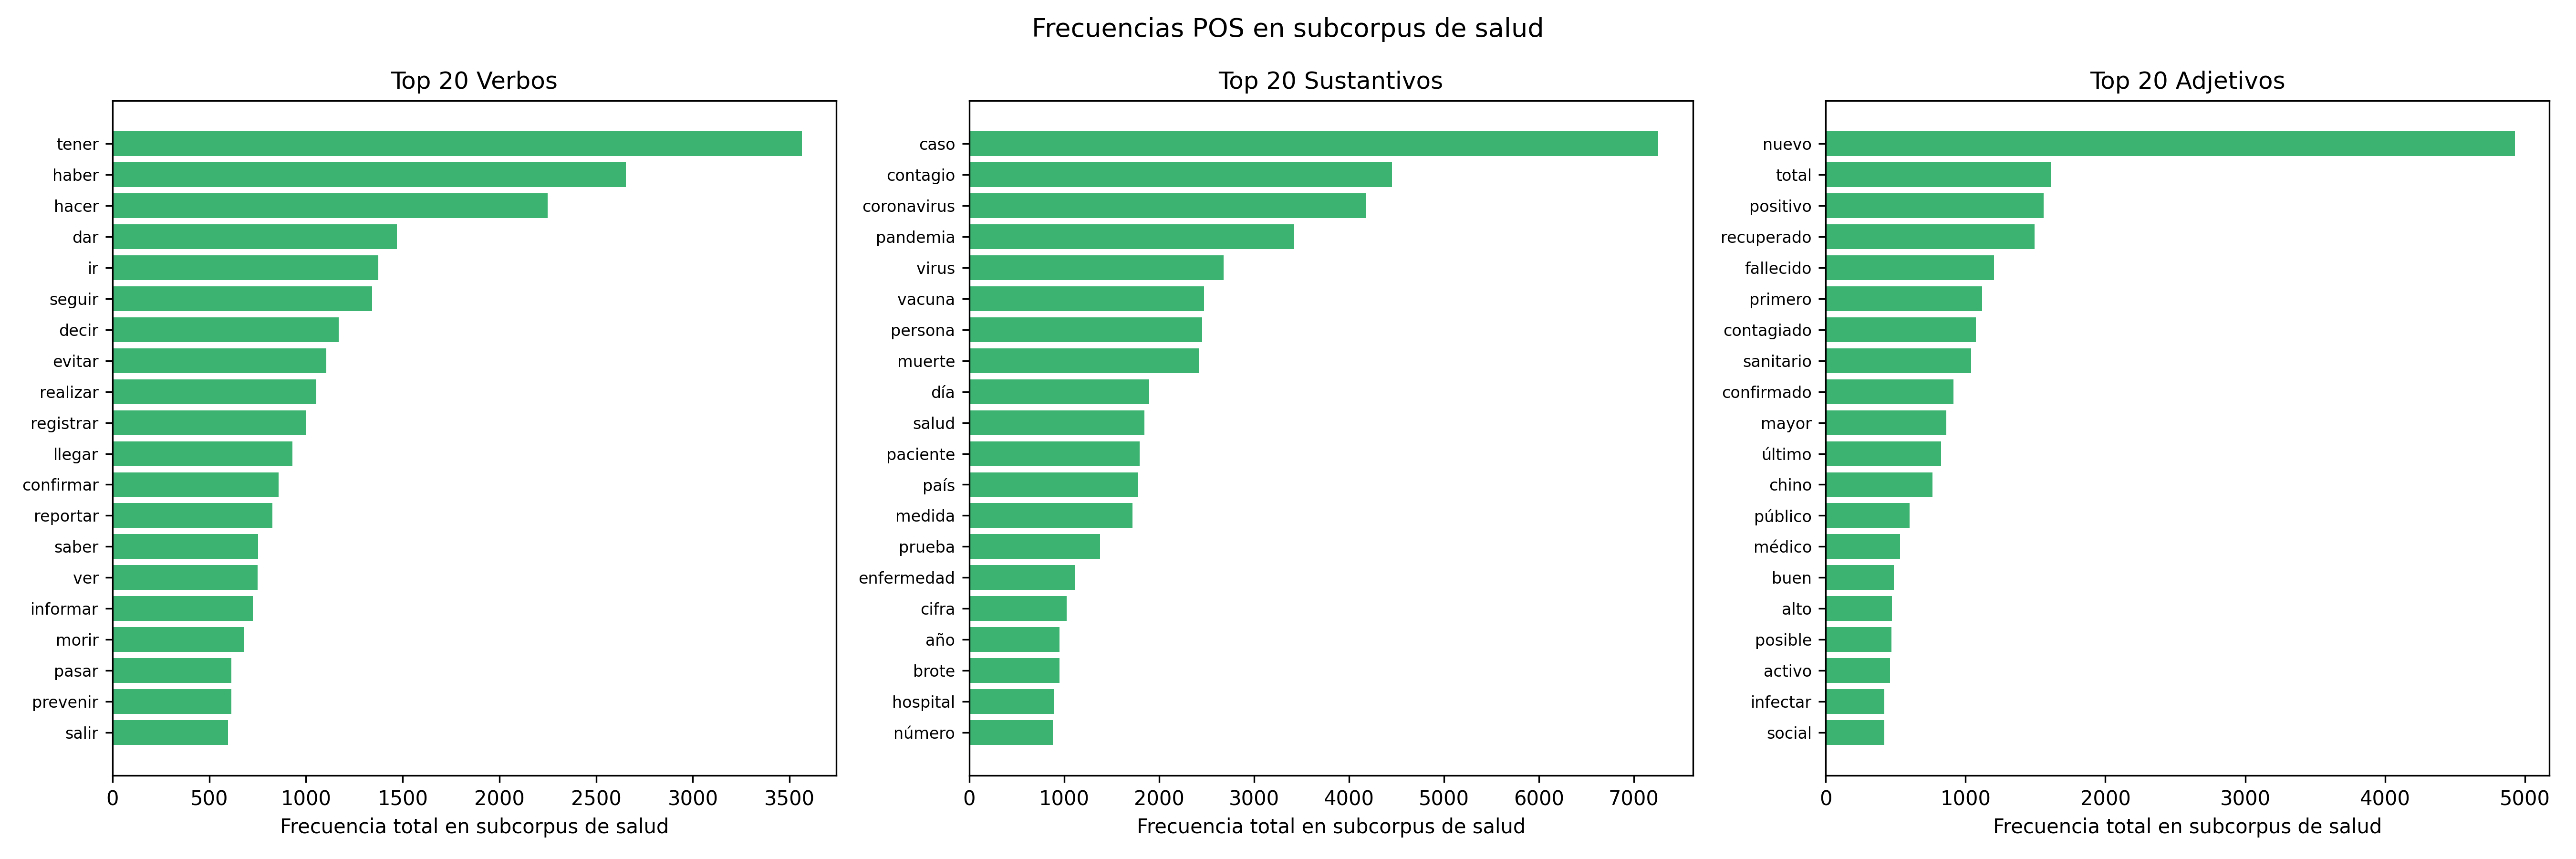
\includegraphics[width=\linewidth]{fig_pos_top_palabras_salud.png}
  \end{figure}

  \begin{center}
  \small
  Top 20 verbos, sustantivos y adjetivos m\'as frecuentes,
  obtenidos mediante an\'alisis morfosint\'actico (Stanza).
  \end{center}

\end{frame}

% ---------------------------------------------------
% Diapositiva 12: Enfermedades y medicamentos
\begin{frame}{Enfermedades y medicamentos mencionados}

  \begin{columns}[T]
    \column{0.5\textwidth}
      \begin{figure}
        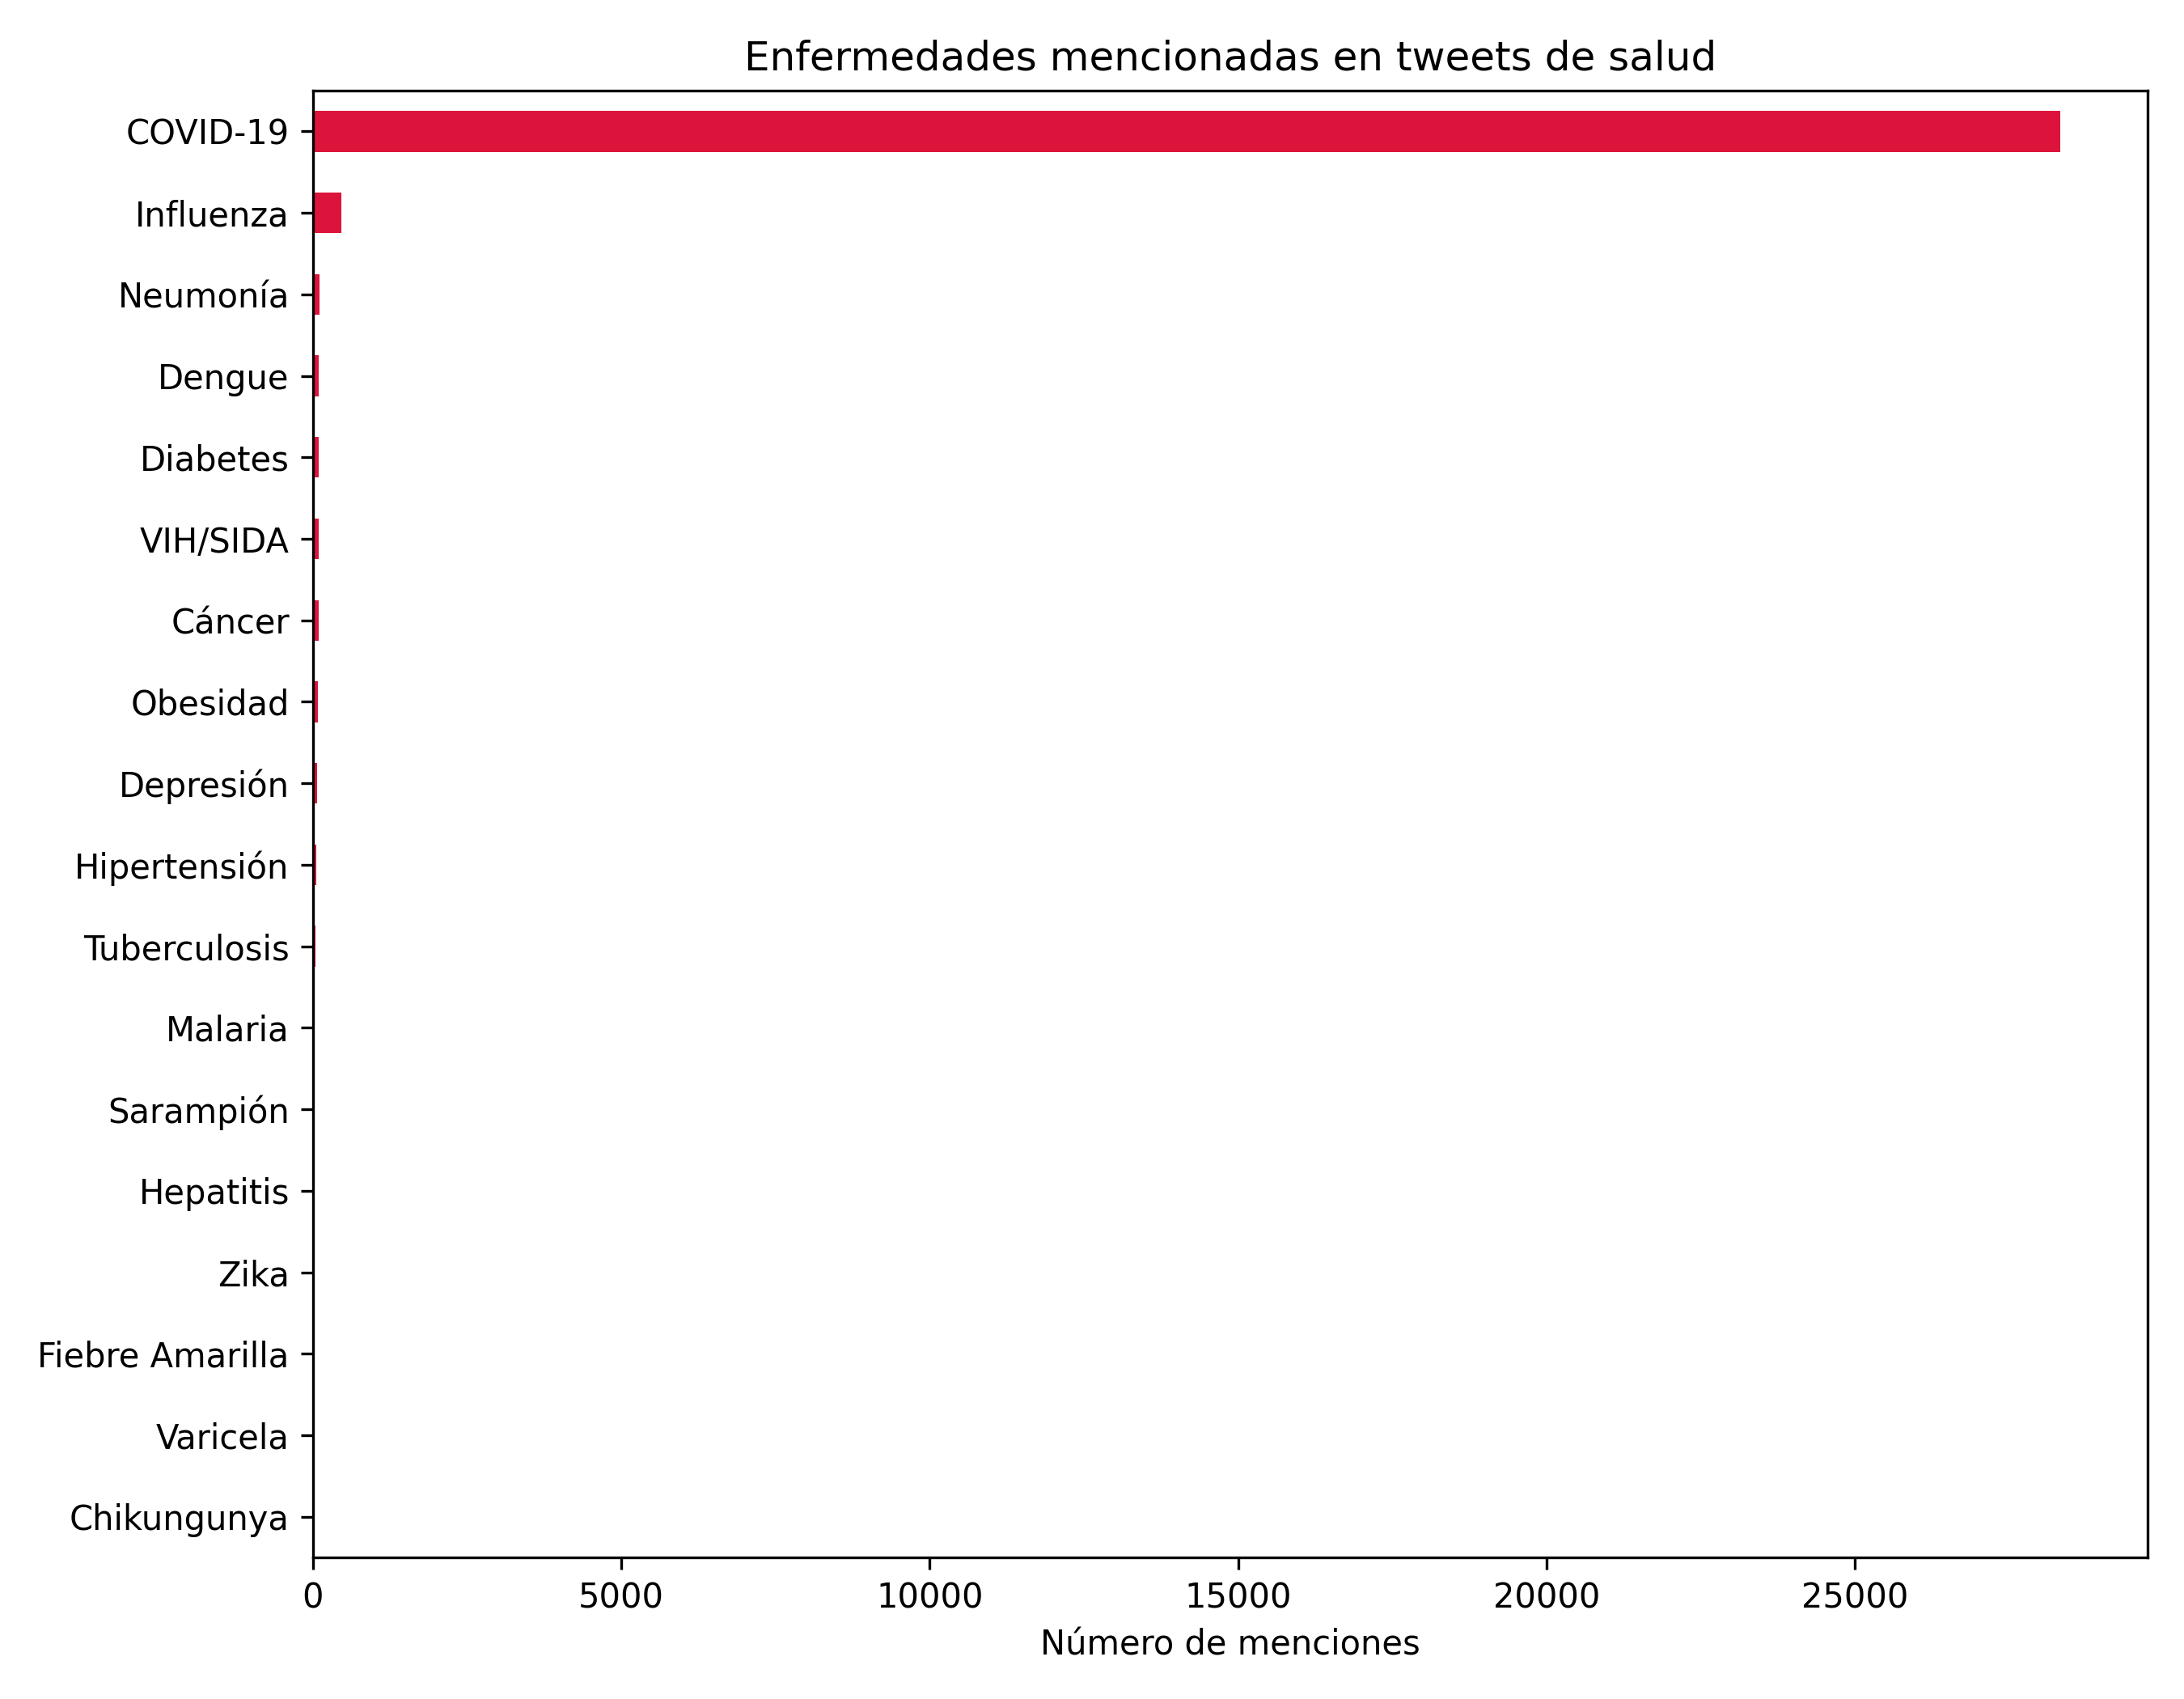
\includegraphics[width=\linewidth]{fig_top_enfermedades_salud.png}
      \end{figure}

    \column{0.5\textwidth}
      \begin{figure}
        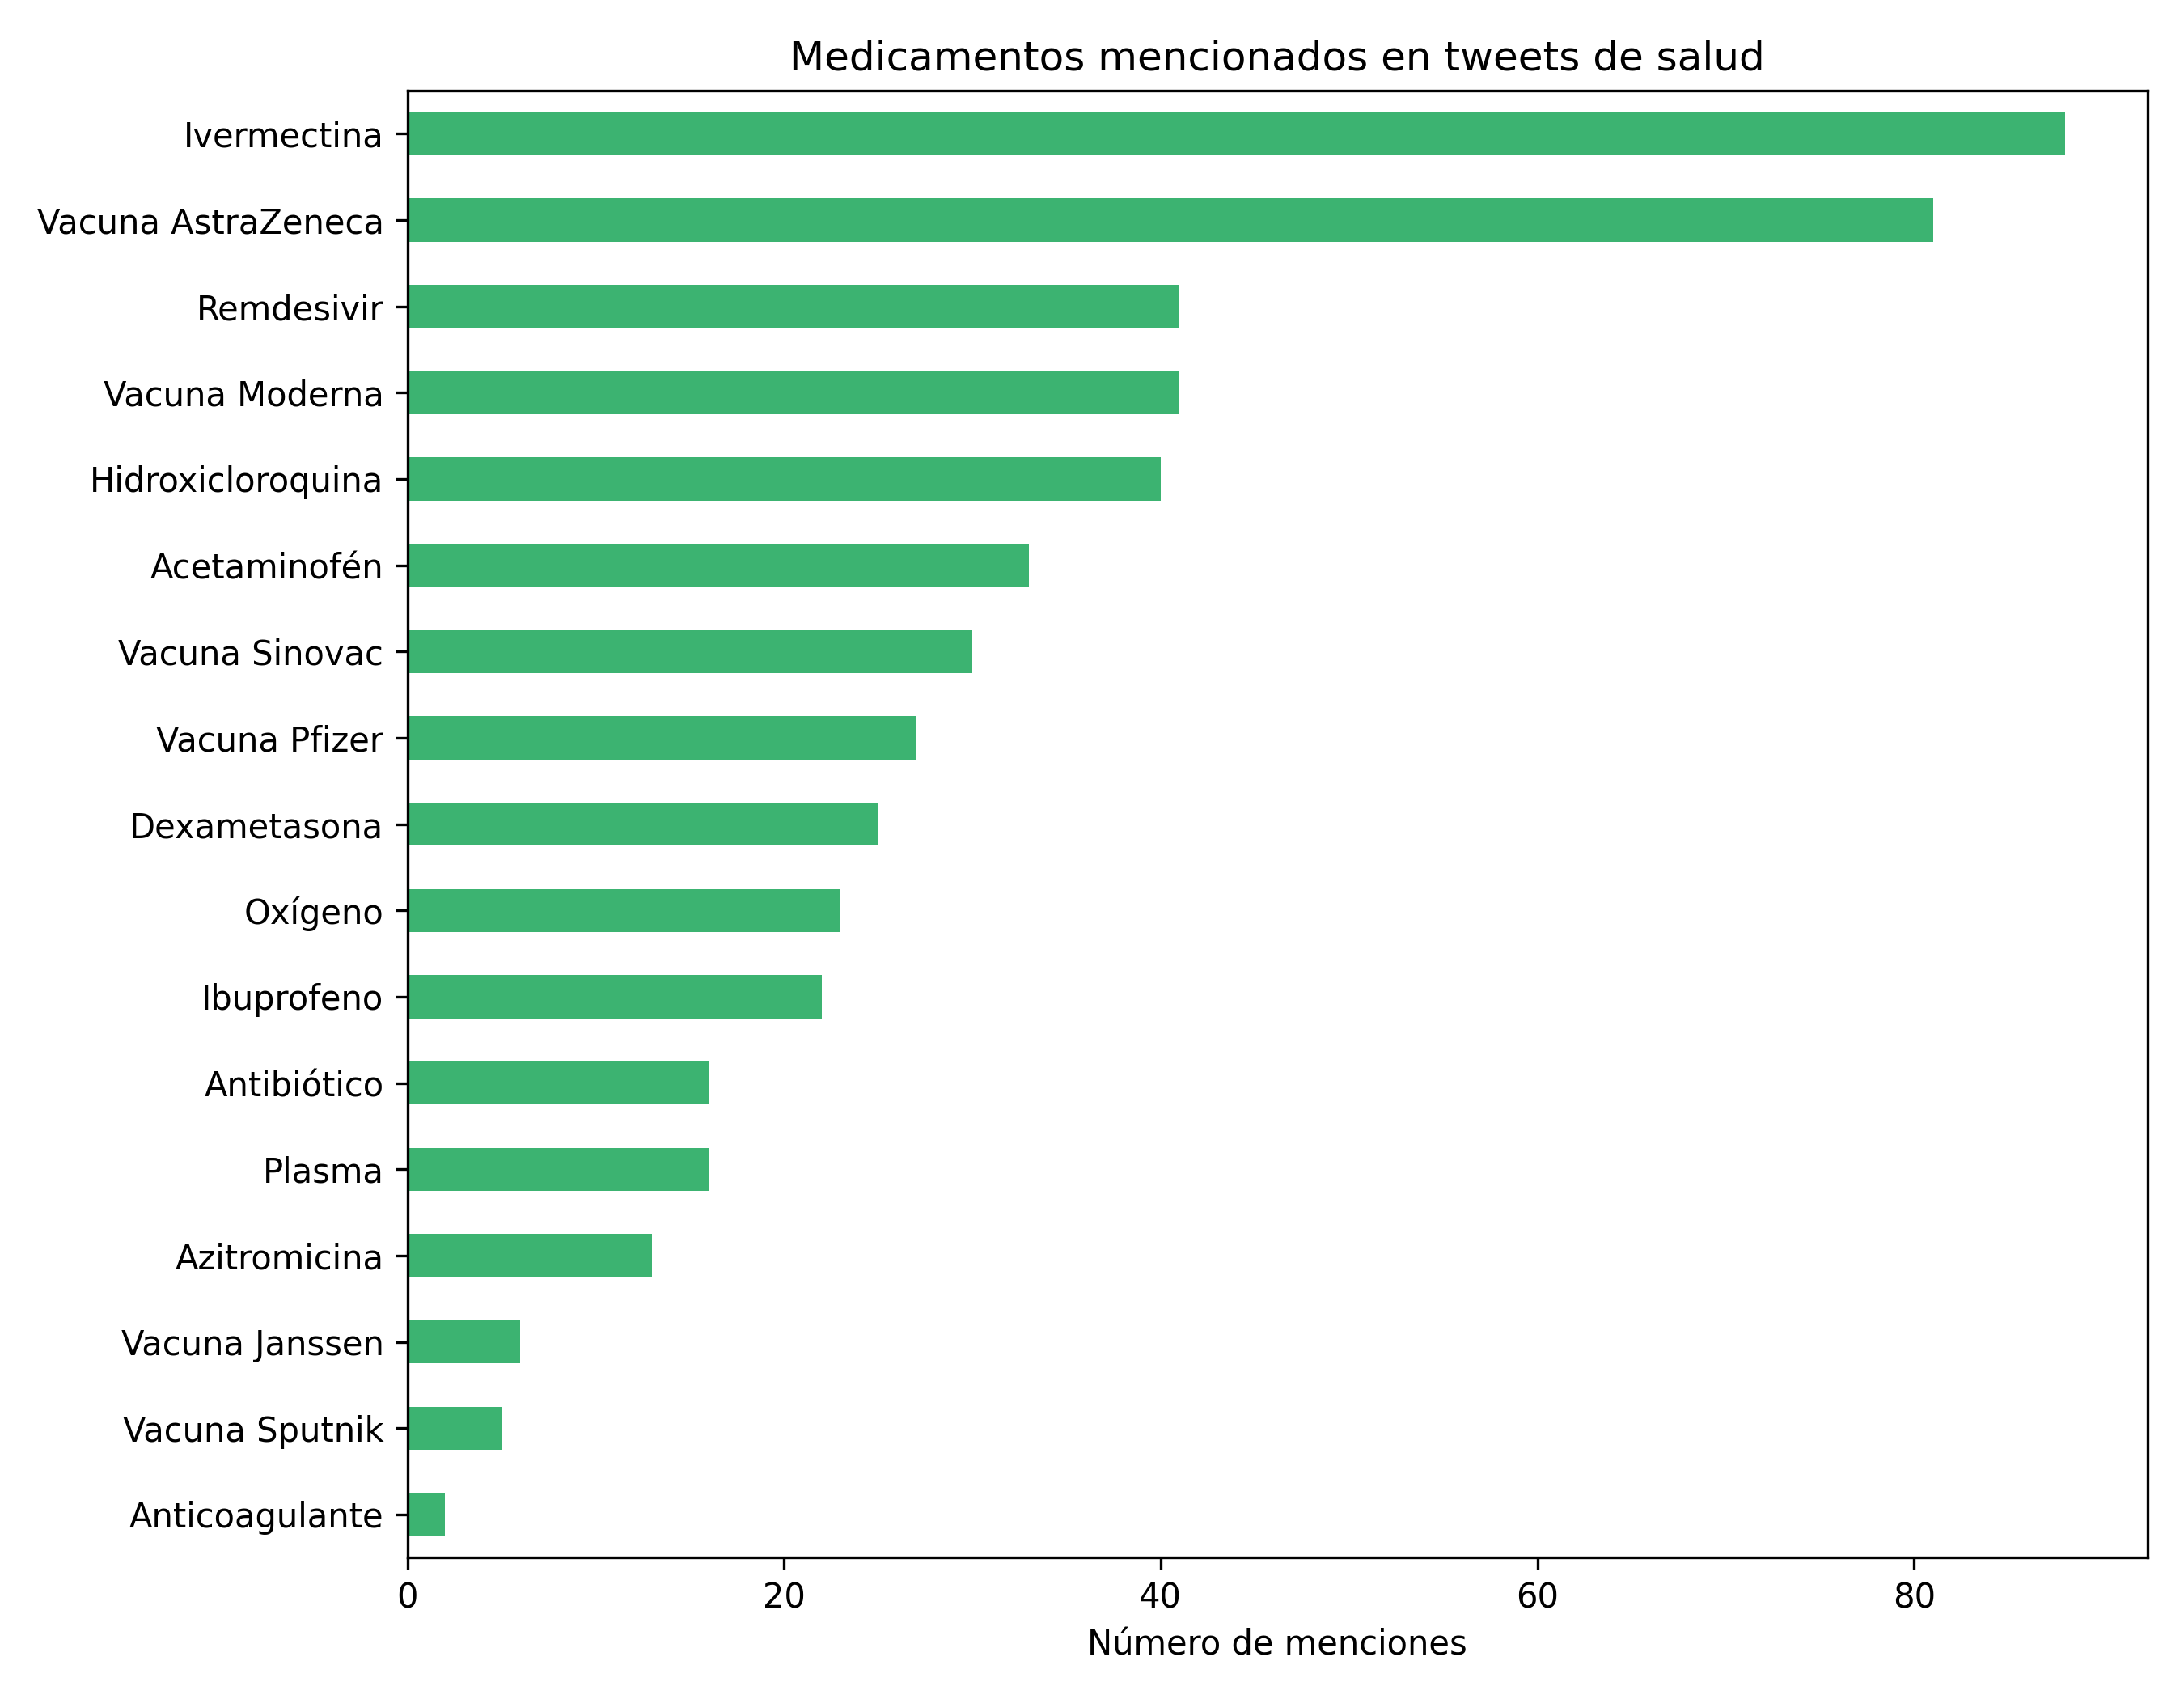
\includegraphics[width=\linewidth]{fig_top_medicamentos_salud.png}
      \end{figure}
  \end{columns}

  \medskip
  \begin{itemize}
    \item B\'usqueda por diccionario de enfermedades y
          medicamentos mencionados en el subcorpus de salud.
    \item Refleja los temas de salud que m\'as resonancia
          tuvieron en la conversaci\'on p\'ublica.
  \end{itemize}

\end{frame}

% ---------------------------------------------------
% Diapositiva 13: Coocurrencias con 'salud'
\begin{frame}{Entidades asociadas a ``salud'' (2020)}

  \begin{figure}
    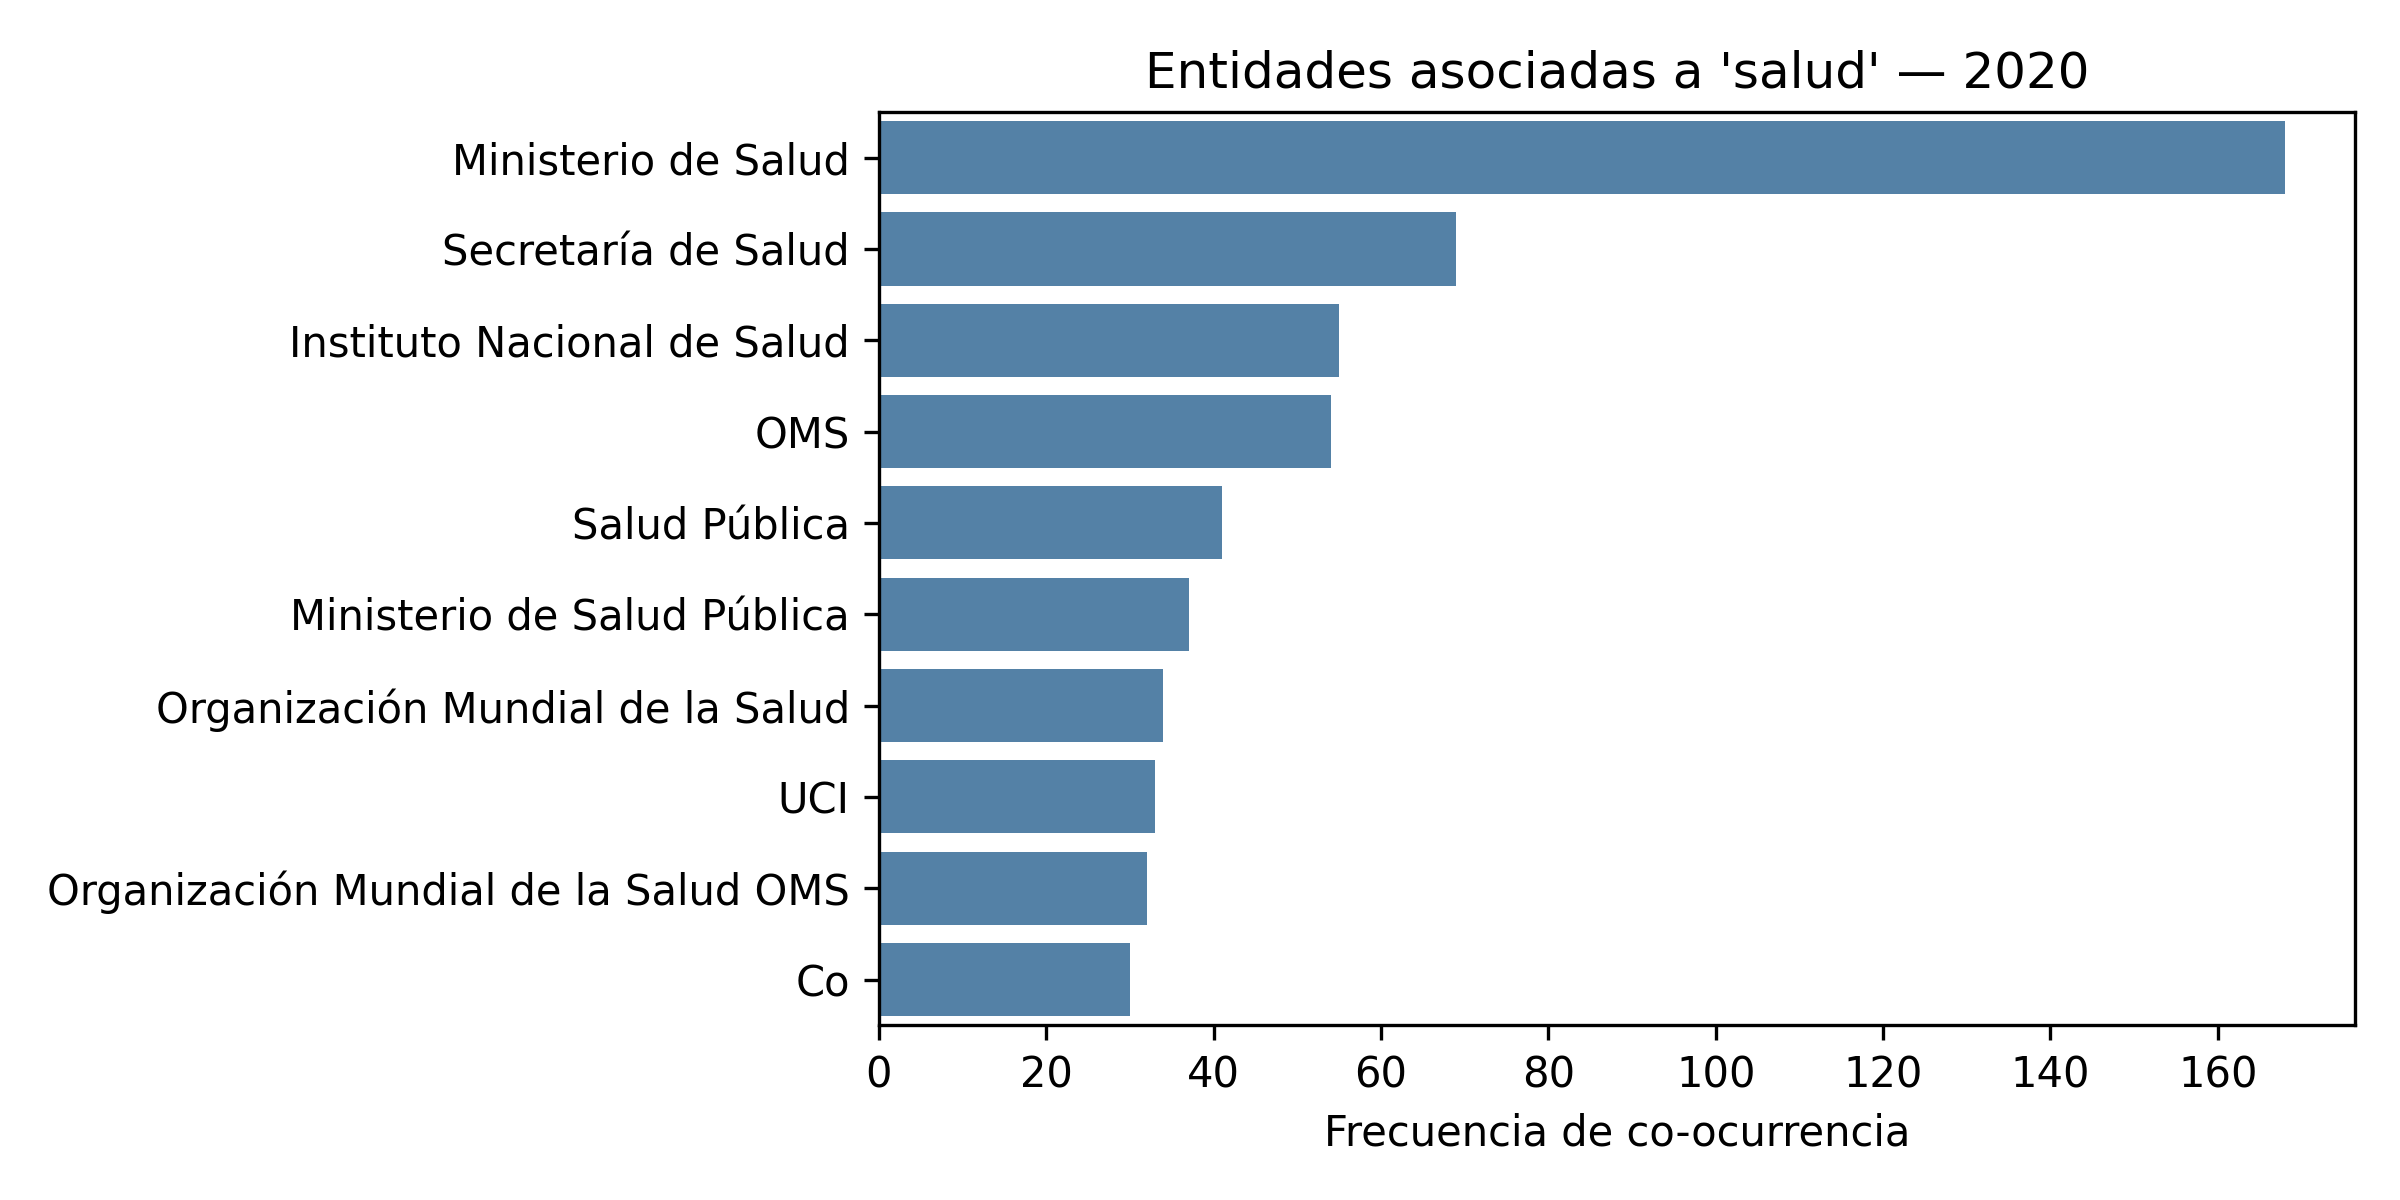
\includegraphics[width=0.6\linewidth]{fig_coocurrencias_salud_2020.png}
  \end{figure}

  \begin{center}
  \small
  Personas y organizaciones (PER/ORG) que m\'as co-ocurren
  con la palabra ``salud'' durante 2020, a\~no marcado por
  la pandemia de COVID-19.
  \end{center}

\end{frame}

% ---------------------------------------------------
% Diapositiva 14: Grafo de red
\begin{frame}{Red de entidades asociadas a ``salud'' (2020)}

  \begin{columns}[T]
    \column{0.55\textwidth}
      \begin{figure}
        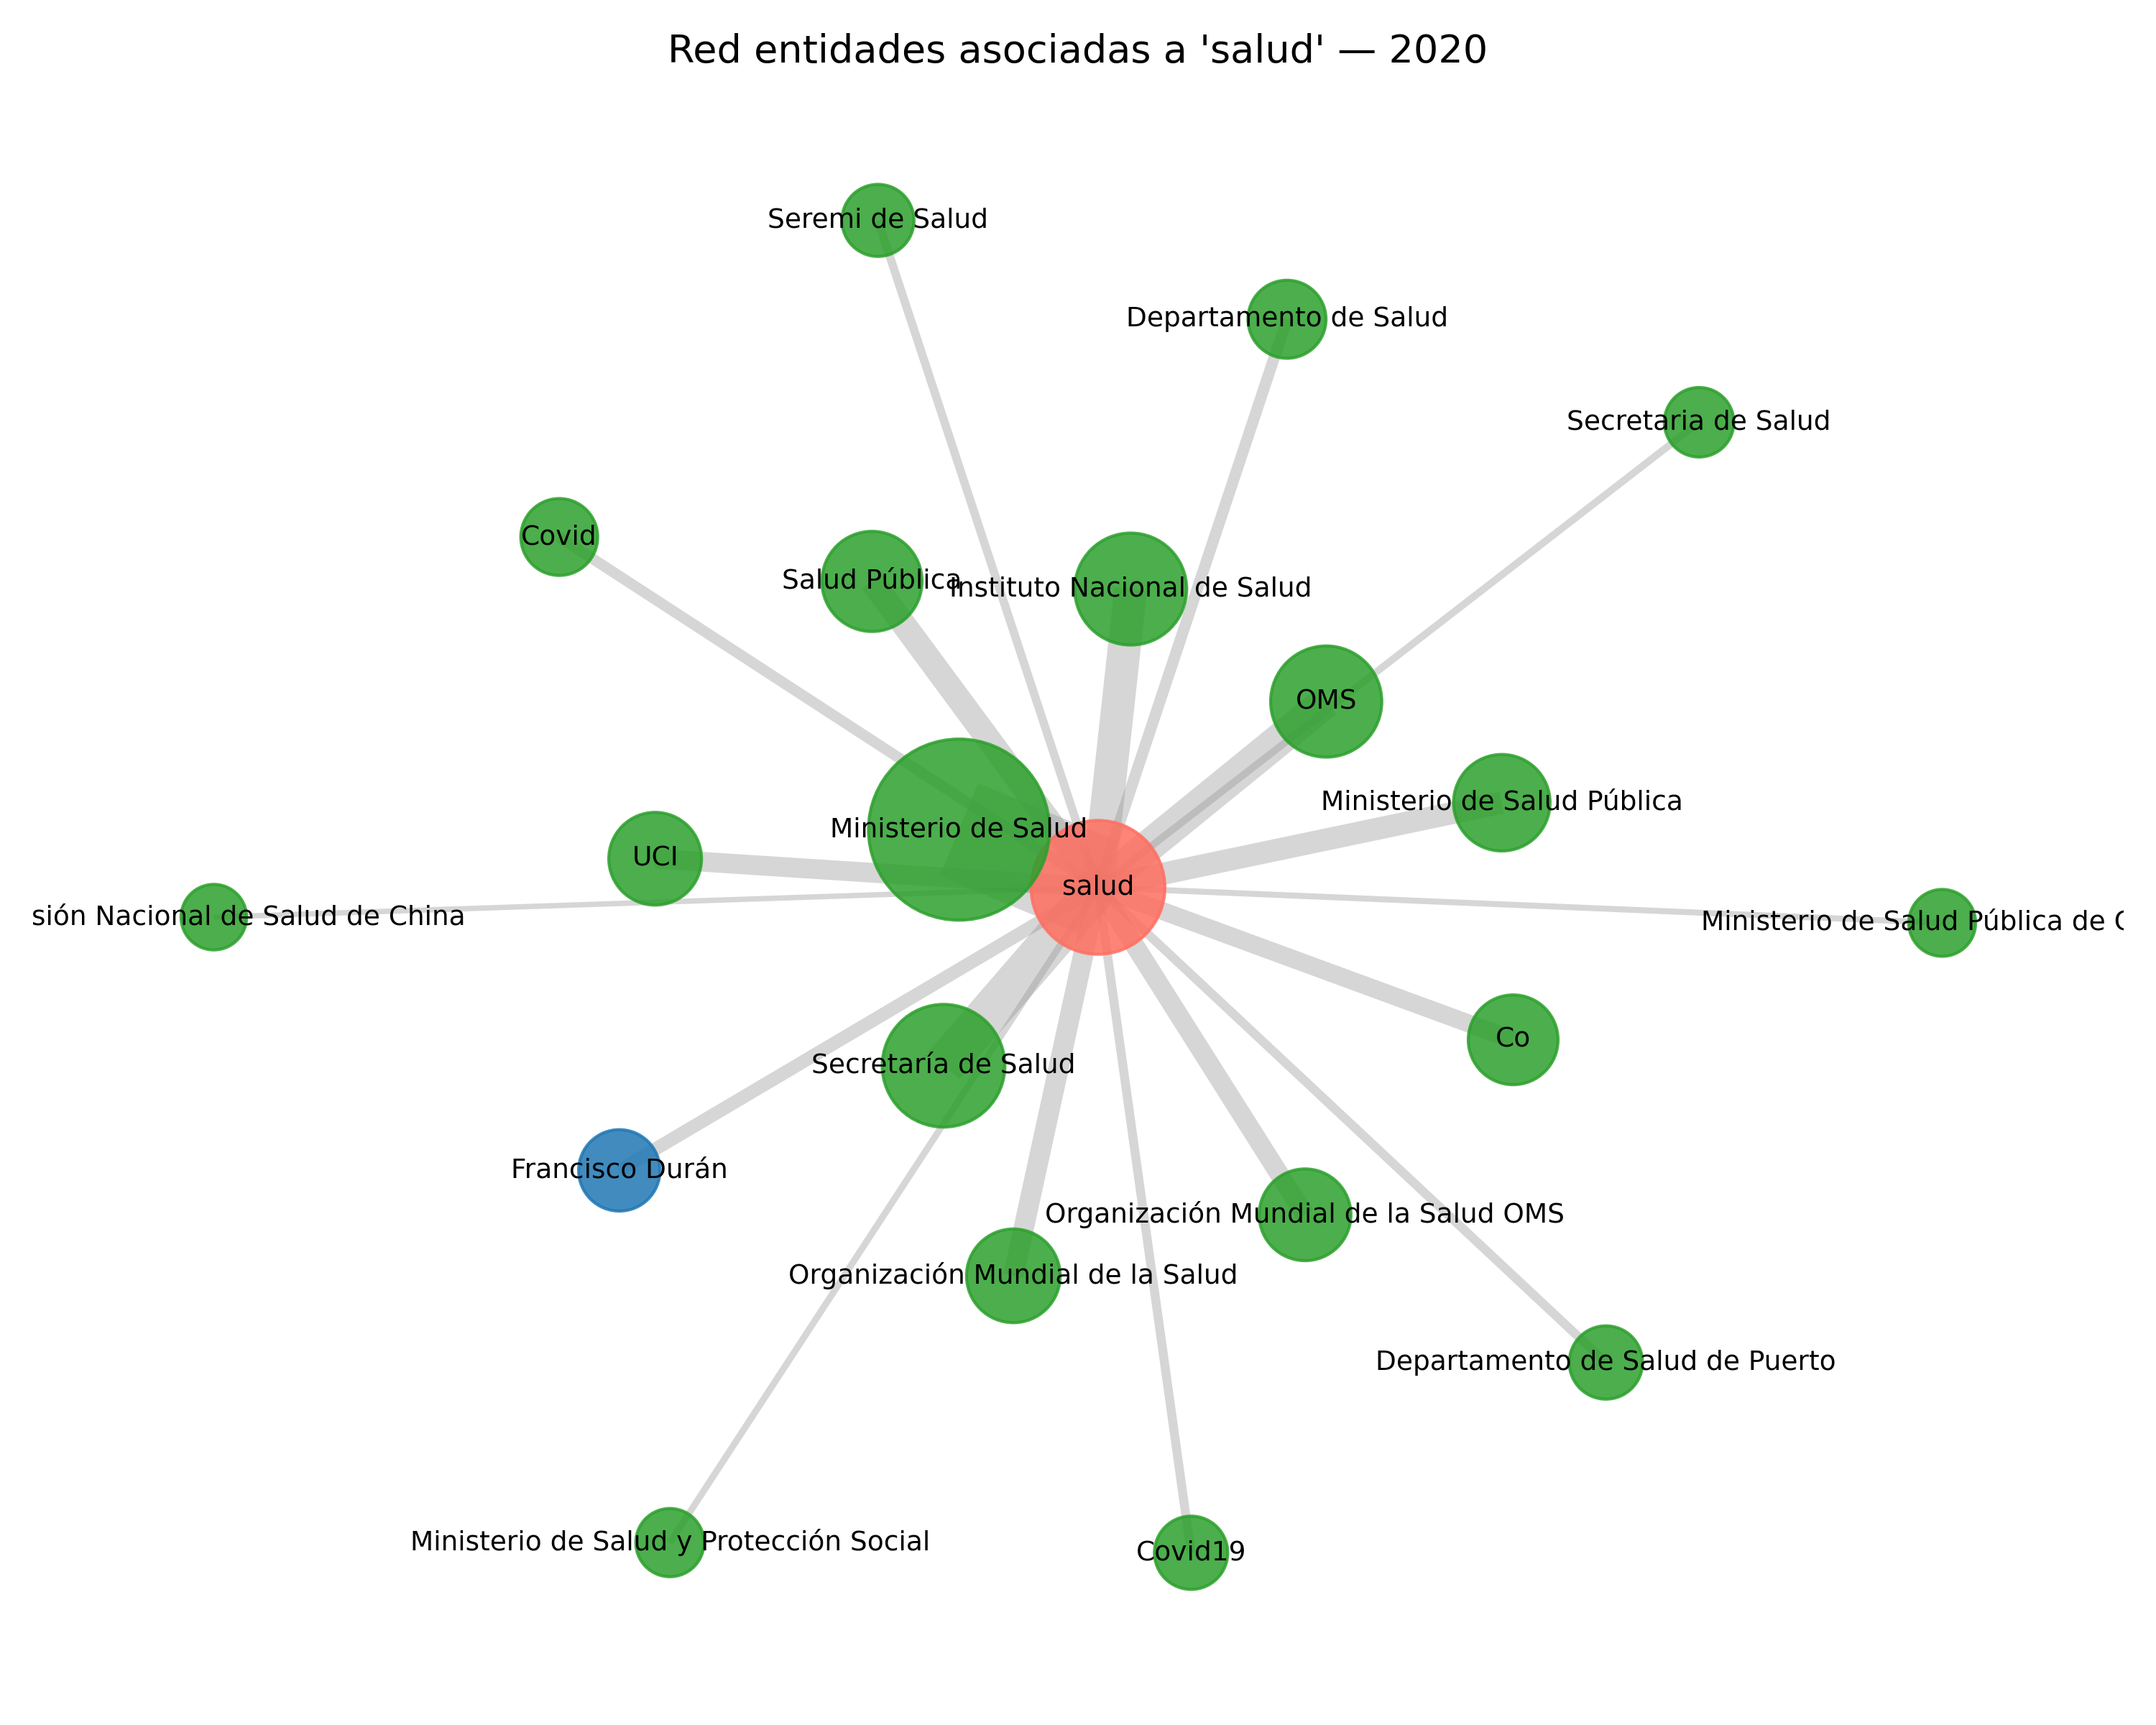
\includegraphics[width=\linewidth]{fig_grafo_salud_2020.png}
      \end{figure}

    \column{0.4\textwidth}
      \textbf{Lectura del grafo}\\[6pt]
      \begin{itemize}
        \item Nodo central (rojo): la palabra ``salud''.
        \item Nodos azules: personas (PER).
        \item Nodos verdes: organizaciones (ORG).
        \item El tama\~no del nodo y el grosor de la
              conexi\'on reflejan la frecuencia de
              co-ocurrencia.
      \end{itemize}
  \end{columns}

\end{frame}

% ---------------------------------------------------
% Diapositiva 15: Conclusiones
\begin{frame}{Conclusiones}

  \begin{columns}[T]
    \column{0.48\textwidth}
      \textbf{Hallazgos principales}
      \begin{itemize}
        \item La conversaci\'on sobre salud se concentra
              en un n\'umero reducido de autores e
              instituciones.
        \item La actividad var\'ia notablemente en el
              tiempo, con picos vinculados a coyunturas
              de salud p\'ublica.
        \item Los temas de salud cubren un conjunto
              amplio de subcategor\'ias, enfermedades
              y medicamentos espec\'ificos.
      \end{itemize}

    \column{0.48\textwidth}
      \textbf{Pr\'oximos pasos}
      \begin{itemize}
        \item Profundizar en el an\'alisis de t\'opicos
              (BERTopic) por subcategor\'ia.
        \item Comparar resultados de salud con los de
              comportamientos protectores.
        \item Explorar relaciones causales entre
              cobertura medi\'atica y comportamiento
              de la audiencia.
      \end{itemize}
  \end{columns}

\end{frame}

\end{document}
